\documentclass [a4paper, 11pt]{article}

\usepackage[utf8]{inputenc}
\usepackage[T1]{fontenc}
\usepackage[portuguese]{babel}
\usepackage{graphicx}
\usepackage{hyperref}
\usepackage{amsmath}
\usepackage{fancyvrb}
\usepackage{listings}
\usepackage{color}
\usepackage{subcaption}
\usepackage{float}

\definecolor{dkgreen}{rgb}{0,0.6,0}
\definecolor{gray}{rgb}{0.5,0.5,0.5}
\definecolor{mauve}{rgb}{0.58,0,0.82}

\lstset{frame=tb,
   language=Python,
   aboveskip=3mm,
   belowskip=3mm,
   showstringspaces=false,
   columns=flexible,
   basicstyle={\small\ttfamily},
   numbers=none,
   numberstyle=\tiny\color{gray},
   keywordstyle=\color{blue},
   commentstyle=\color{dkgreen},
   stringstyle=\color{mauve},
   breaklines=true,
   breakatwhitespace=true
   tabsize=3
   }
   
\renewcommand{\lstlistingname}{Algoritmo}

\title{Trabalho Prático 2}
\author{Universidade Federal de Minas Gerais \\ Departamento de Ciência da Computação \\ Computação Natural \\ \\ João Francisco Barreto da Silva Martins \\ \texttt{<joaofbsm@dcc.ufmg.br>}}

\begin{document}
\maketitle

\section{Introdução}

O problema das p-medianas é um problema de localização de instalações, também conhecidos como análise de localização, um ramo da Pesquisa Operacional. Esse problema consiste em localizar $p$ centros(medianas) em um grafo totalmente conectado a fim de minimizar a soma da distância de cada vértice ao seu centro mais próximo. Uma representação gráfica do problema pode ser vista na Figura \ref{fig:p-medians}.

\begin{figure}[h]	
  \centering
  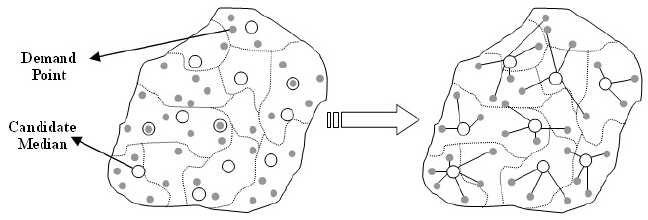
\includegraphics[width=10cm,keepaspectratio]{images/p-medians.png}
  \caption{Representação gráfica do problema das p-medianas.}
  \label{fig:p-medians}
\end{figure}

O objetivo desse trabalho é resolver o problema das p-medianas com restrições de capacidade, onde cada nó possui uma capacidade total e uma demanda por recursos pré-determinada. Ambos os problemas se encontram na categoria NP-difícil. Os detalhes técnicos e experimentais dessa implementação serão discutidos ao longo deste documento.


\section{Modelagem e Implementação}

A linguagem escolhida para implementação foi Python 3(versão 3.6.0), por apresentar diversas funcionalidades de alto nível já implementadas, assim me dando a liberdade necessária para que eu pudesse focar mais nos detalhes realmente importantes da implementação. O código do trabalho pode ser encontrado em \url{https://github.com/joaofbsm/p-medians}. 

Toda a implementação foi baseada no artigo de França et al \cite{de2005max}. Esse artigo descreve um \textit{Min Max Ant System}(MMAS) modificado e adequado para resolver o problema das p-medianas com restrições de capacidades. Alguns problemas foram encontrados na descrição da implementação, presente no artigo, e esse fatores serão discutidos mais para frente. 

\subsection{Representação do mundo}

O mundo no qual o problema está inserido foi modelado com um vetor de entidades \textbf{Node}, que possuem uma posição no espaço bidimensional, uma capacidade, uma demanda e um nível de feromônios, e uma matriz de distâncias euclidiana entre os nós, onde os nós são indexados de acordo com sua posição no vetor inicialmente citado. 

\subsection{Heurística de informação}

\cite{de2005max} apresenta uma heurística de informação, baseada na densidade de clusters ao redor dos nós, a fim de melhorar a solução do sistema. Ela diz respeito à qualidade de escolha de cada nó como parte da solução, e é usada no momento de escolha das medianas. O pseudocódigo para geração do vetor com as densidades é mostrado na subseção 4.2 do artigo.

\subsection{Escolha das medianas}

A escolha das medianas é o primeiro passo do algoritmo, que, para este fim, faz o uso de um algoritmo de otimização de colônia de formigas(ACO) conhecido como \textit{Min Max Ant System}(MMAS). Esse sistema difere de um \textit{Ant System} clássico pois impõe \textit{thresholds} inferiores(min) e superiores(max) nos valores dos feromônios. Os valores mínimo($\tau_{min}$) e máximo($\tau_{max}$) são setados para 0.001 e 0.999, respectivamente, e o valor inicial para 0.5, como especificado em \cite{de2005max}. Os feromônios nessa implementação ficam nos nós, e não nas arestas como no ACO clássico.

Na seção 3.1 de \cite{de2005max} é apresentado o algoritmo para um \textit{Ant System}, no entanto um para o MMAS nunca é mostrado. O pseudocódigo seguido na implementação do MMAS é descrito no Algoritmo \ref{alg:mmas}

\medskip
\begin{lstlisting}[label=alg:mmas, caption=Pseudocódigo para o Min Max Ant System.]
	def MMAS(world, colony):
    	world.reset_pheromones(initial_pheromone)
        global_best = Solution(distance=inf)
        for i in range(n_iterations):
        	for ant in colony.ants:
            	ant.build_solution(world)
            best, worst = evaluate_solutions(world, colony)
            world.update_pheromones(decay, global_best, best, worst)
            if is_stagnated(world, max_pheromone, min_pheromone):
            	world.reset_pheromones(initial_pheromone)
            if best.distance < global_best.distance:
            	global_best = best
              
\end{lstlisting}
\medskip

Ao chamarmos \texttt{build\_solution}, utilizamos cada formiga na colônia para gerar uma solução. Uma formiga escolhe $p$ entre $n$ pontos totais para se tornarem medianas. A escolha é feita de forma probabilística e a cada iteração o nó escolhido é retirado do cálculo. A probabilidade de escolha de um nó é calculada como descrito a seguir:

\begin{figure}[H]	
  \centering
  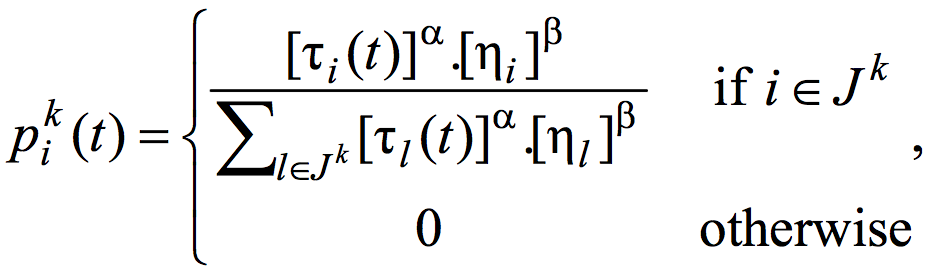
\includegraphics[width=5.3cm,keepaspectratio]{images/probabilities.png}
\end{figure}

onde $\alpha$ e $\beta$ são parâmetros definidos pelo usuário para controlar o peso da trilha de feromônios $\theta_i(t)$, com $i$ sendo o nó e $t$ a iteração corrente, e da heurística de informação $\eta_i$ no cálculo da probabilidade de escolha de um nó.

\texttt{evaluate\_solutions} avalia as soluções geradas ao atribuir os nós às medianas usando a heurística construtiva para o GAP, explorada melhor na subseção \ref{sub:gap}. As funções \texttt{update\_pheromones} e \texttt{is\_stagnated} são discutidas nas subseções \ref{sub:update-pheromone} e \ref{sub:stagnation}, respectivamente.

\subsection{Heurística para GAP} \label{sub:gap}
\textit{General Assignment Problem}(GAP) é um problema de otimização combinatória, sendo a generalização do problema de atribuição. O GAP pode ser descrito como a atribuição de um número de agentes à um número de tarefas, visando maximizar um ganho. No problema em questão ele visa minimizar a seguinte função objetivo:

\begin{figure}[H]	
  \centering
  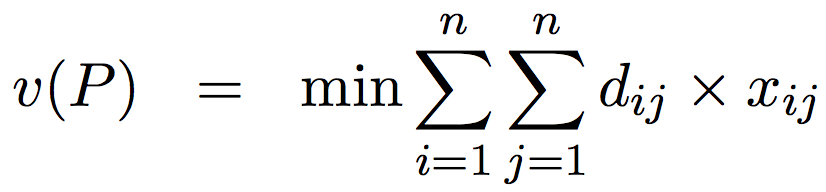
\includegraphics[width=4cm,keepaspectratio]{images/objective_function.png}
\end{figure}

onde $n$ é o número de vértices na rede, $P$ é o número de centros (medianas) a serem
localizados e $[d_{ij}] n \times n$ é uma matriz de custos (distâncias). Além disso temos uma matriz de associação entre os nós descrita como:

\begin{figure}[H]	
  \centering
  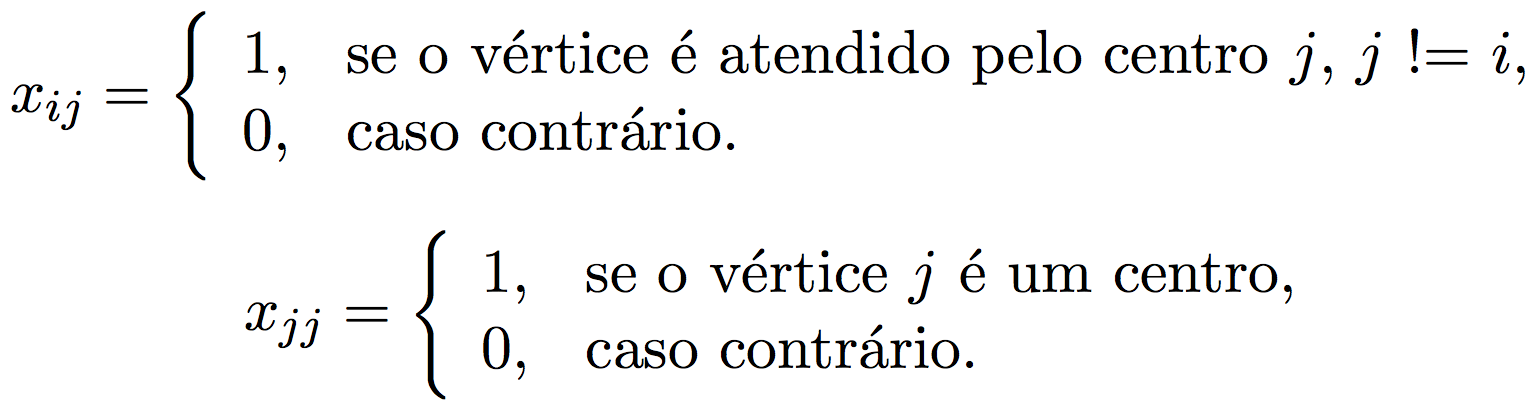
\includegraphics[width=7.5cm,keepaspectratio]{images/association.png}
\end{figure}

\cite{de2005max} apresenta uma heurística construtiva para solução do GAP na subseção 4.1, a qual foi reproduzida na Figura \ref{fig:gap}. No entanto, essa heurística não está correta, pois ela acaba gerando muitas soluções inválidas, uma vez que, com frequência, existem nós que não conseguem ser atribuídos a nenhuma mediana por problemas de excesso de capacidade. Portanto foi feita uma alteração na mesma, para que, ao ordenarmos os clientes, ao invés de usarmos a distância como fator, usamos a demanda de cada nó, em ordem decrescente. 

\begin{figure}[h]	
  \centering
  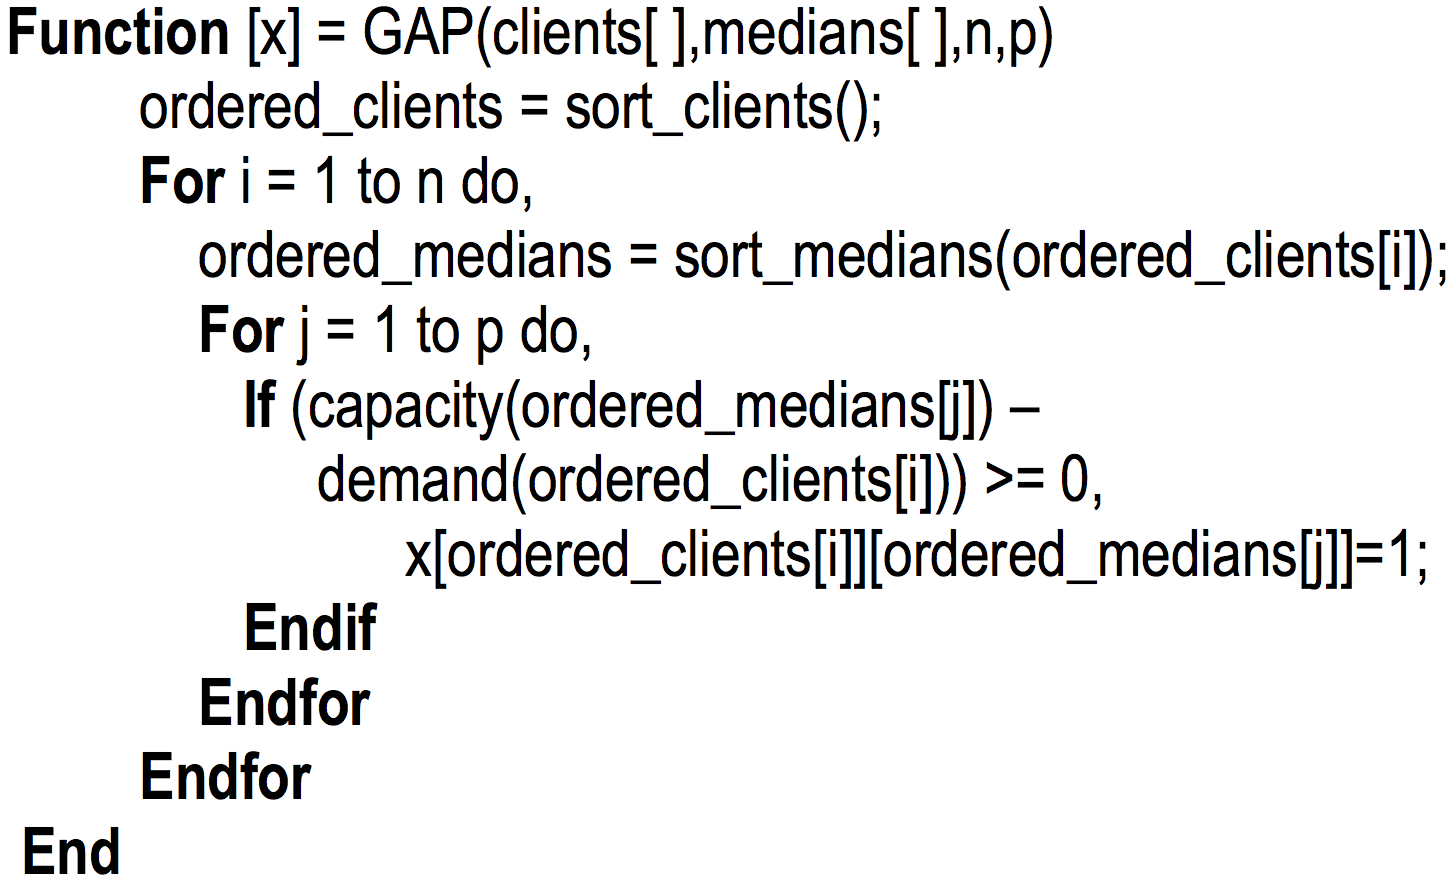
\includegraphics[width=7cm,keepaspectratio]{images/gap.png}
  \caption{Heurística construtiva para alocação de clientes às medianas.}
  \label{fig:gap}
\end{figure}

Com a alteração não chegamos na situação onde um cliente $c$ de demanda $d$ não consegue ser atribuído a nenhum centro, pois, apesar da soma da capacidade restante de todos os centros ser maior do que $d$, nenhum deles possuí, individualmente, capacidade restante para aceitar $c$, uma vez que a capacidade deles já foi consumida por outros clientes anteriormente.

Ao fim da execução da heurística retornamos uma matriz de associação dos nós $x$.

\subsection{Atualização dos feromônios} \label{sub:update-pheromone}

Após a avaliação das soluções geradas para aquela iteração, é o momento de atualizar o feromônios nos nós da rede. Eles são atualizados de acordo com a fórmula:

\begin{figure}[H]	
  \centering
  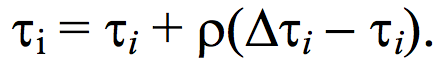
\includegraphics[width=3cm,keepaspectratio]{images/phero_update.png}
\end{figure}

onde $\rho$ é a taxa de evaporação do feromônio e $\Delta\tau_i$ é taxa de atualização do feromônio, calculada a cada iteração como:

\begin{figure}[H]	
  \centering
  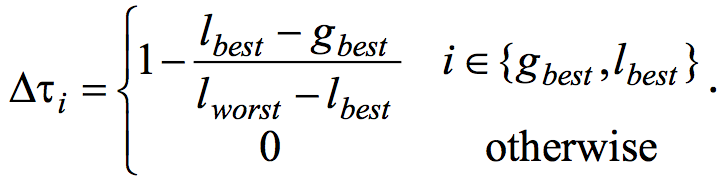
\includegraphics[width=6cm,keepaspectratio]{images/delta_t.png}
\end{figure}

onde $g_best$, $l_best$ e $l_worst$ são os valores totais das distâncias entre os nós na melhor solução global, melhor solução local e pior solução local, respectivamente. Como consequência dessa fórmula mantemos os feromônios nos thresholds setados anteriormente. 

Assim que atualizados os feromônios, a melhor solução global pode ser atualizada, caso seja esse o caso.

\subsection{Controle de estagnação} \label{sub:stagnation}

Como consequência do MMAS, é possível que após certo número de iterações o sistema estagne em suas soluções, com $p$ nós apresentando feromônio igual a $\tau_{max}$, e os restantes $n - p$ nós apresentando feromônios iguais a $\tau_{max}$. A estagnação pode ser detectada com a equação:

\begin{figure}[H]	
  \centering
  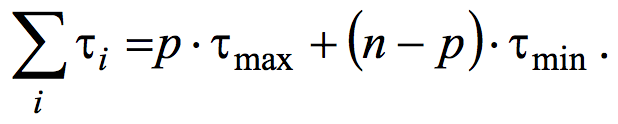
\includegraphics[width=4.5cm,keepaspectratio]{images/stagnation.png}
\end{figure}

Caso os dois lados da equação sejam iguais, os feromônios são resetados para o valor inicial, no entanto mantendo a melhor solução global armazenada.

\subsection{Otimização do código}
Python não é nem de longe a melhor linguagem de programação para se implementar problemas de otimização e de aprendizado de máquina, pois estes são problemas que exigem muito processamento. Processamento é o principal problema enfrentado por Python, por abstrair muitos dos detalhes computacionais, além de ser interpretada ao invés de compilada. 

Para que a execução dos experimentos se desse de forma mais rápida então a biblioteca \texttt{NumPy}, cuja utilização se dá em C, foi amplamente utilizada, com a maioria das operações iterativas tendo sido adaptadas para cálculos com matrizes. A biblioteca \texttt{Cython} também foi utilizada em 3 dos módulos criar para gerar diretamente código C, assim também agilizando o processo de execução. Com todas essas mudanças o código passou a rodar 2.5 vezes mais rápido no total.

Para que o código Cython(extensão .pyx) possa ser executado juntamente com o código em Python(extensão .py) é necessário antes executar o script auxiliar \texttt{setup.py} da seguinte forma:

\begin{center}
\begin{verbatim}
    python3 setup.py build_ext --inplace
\end{verbatim}
\end{center}


\section{Análise Experimental}

Por se tratar de um problema de otimização combinatória, rodamos cada experimento com 30 repetições. Todos os testes foram feitos em máquinas da Google através da plataforma Google Cloud. Os parâmetros variados nas execuções estão descritos na seção \ref{xp_par}. A análise experimental dos três \textit{datasets} estão divididas nas subseções seguintes.

O código pode ser executado pela linha de comando com os seguintes argumentos:

\begin{center}
\begin{verbatim}
    python3 main.py [-i ITERATIONS] [-a ANTS] [--alpha ALPHA] 
                    [--beta BETA] [--rho RHO] dataset
\end{verbatim}
\end{center}

\subsection{Parâmetros} \label{xp_par}

Os parâmetros são passados como argumentos na chamada do código. São eles:

\begin{itemize}
	\item Número de iterações(\textbf{Padrão}: 50) 
    \item Número de formigas((\textbf{Padrão}: $n - p$)
    \item Alpha(\textbf{Padrão}: 0.5) - Peso do feromônio do nó no cálculo da probabilidade.
    \item Beta(\textbf{Padrão}: 0.5) - Peso da heurística de informação no cálculo da probabilidade.
    \item Rho(\textbf{Padrão}: 0.9) - Taxa de evaporação do feromônio.
\end{itemize}

A semente mestra para o gerador aleatória é $123456$. A partir dela são geradas 30 outras sementes para serem usadas nas repetições. Ao fixarmos as sementes, permitimos que os resultados sejam reproduzíveis, caso necessário.

\subsection{Bases de dados}
3 bases de dados foram disponibilizadas para a realização dos experimentos: SJC1, SJC2 e SJC3b. Todas possuem números diferentes de nós, estes com características diferentes, e de medianas a serem encontradas. Os parâmetros foram variados um por um, sempre mantendo os valores padrões, como apresentados na subseção \ref{xp_par}, para aqueles que ficaram constantes naquela rodada de execuções.

\subsubsection{SJC1}

A base de dados SJC1 é composta de 100 pontos, todos com capacidade 720, mas com demanda variável. Ela busca por 10 pontos de mediana. Inicialmente buscamos entender o impacto do número de iterações no algoritmo. Como podemos ver na Figura \ref{fig:sjc1_iterations}, a medida que as iterações passam, melhor é a solução encontrada, como era de se esperar. 

\begin{figure}[h]	
  \centering
  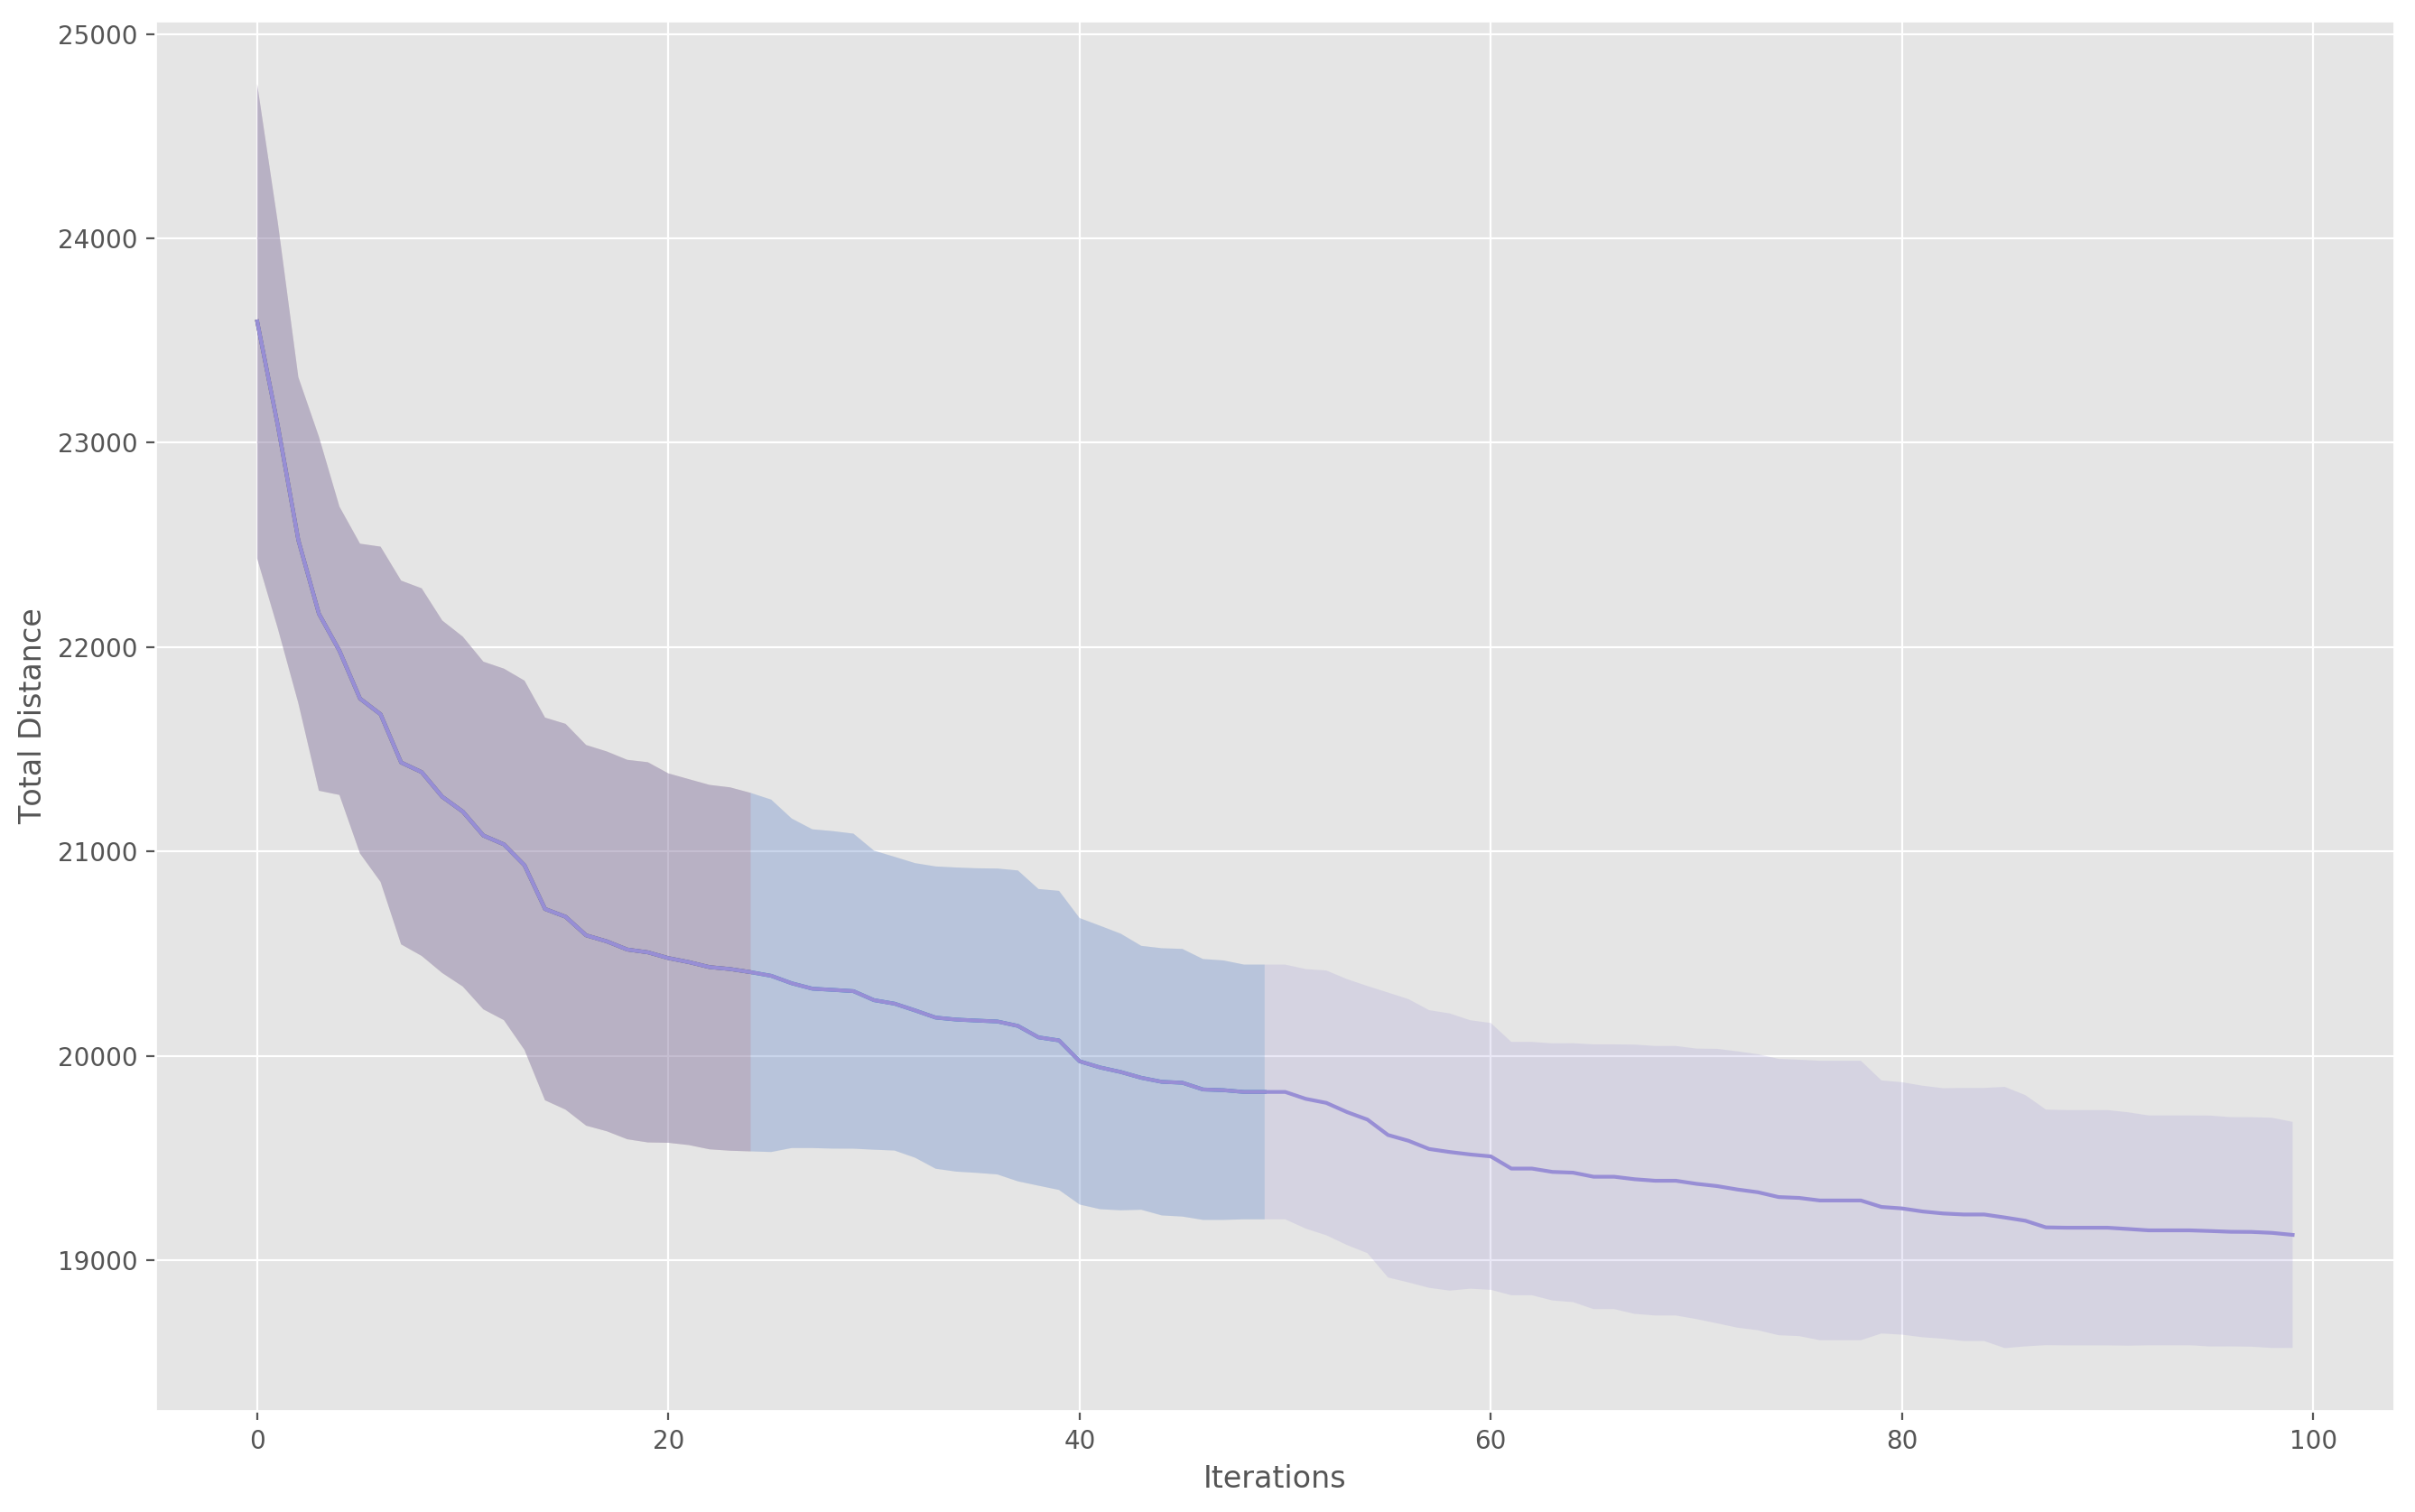
\includegraphics[width=11cm,keepaspectratio]{images/SJC1_iterations.png}
  \caption{Média e desvio padrão para a distância da solução encontrada para base SJC1 com número de iterações variável.}
  \label{fig:sjc1_iterations}
\end{figure}

Agora avaliaremos o que acontece quando variamos o número de formigas, e portanto o número de soluções geradas a cada iteração do algoritmo. Variamos as quantidade de formigas de acordo com $p$, $n - p$ e $2 * (n - p)$. A Figura \ref{fig:sjc1_ants}. Aqui algo inesperado acontece: após a iteração 32, e até a iteração final, tanto a média quanto o desvio padrão sofrem um mudança brusca. Isso aconteceu pois em uma das execuções, após essa iteração, a distância total cai de 21479 para 958. 

Analisando o porque esse foi o caso, chegou-se a conclusão de que o problema está provavelmente na detecção de estagnação presente no artigo. O fato aqui é que, aparentemente, o sistema converge antes do valor somado dos feromônios alcançar o total especificado na fórmula. Para tentar corrigir esse problema, um valor(0.5). para aumentar o \textit{range} de detecção de estagnação, adicionado à fórmula da seguinte forma:

\medskip
\begin{lstlisting}
if total_pheromone >= stagnation_threshold - 0.5:
	is_stagnated = True
\end{lstlisting}
\medskip
    
Esse valor foi encontrado empiricamente e resolveu para muitos casos, falhando raramente. O problema é que quando o sistema estagna, ele gera as mesmas soluções para todas as formigas, ou seja, o melhor e o pior valores locais são os mesmos e portanto a fórmula apresentada na subseção \ref{sub:update-pheromone} fica com um denominador igual a 0, fazendo com o que o algoritmo pare de funcionar corretamente.

Outra hipótese é a de que os valores padrão(0.5) de \textit{alpha} e \textit{beta}, que causam uma radiciação quando utilizados na fórmula da probabilidade, acabam gerando valores inválidos em raras ocasiões, causando o mesmo problema do denominador nulo. É estranho o fato de que nem \cite{de2005max} e nem o próprio criador do ACO, Marco Dorigo, em \cite{dorigo2003ant} citam essa provável ocorrência, o que me leva a acreditar na primeira hipótese.

Ao ignorarmos o resultado errado, encontramos o resultado que era de se esperar nesse teste: quanto mais formigas melhor. Portanto, $2 * (n - p)$ se mostrou o mais eficiente para encontrar soluções melhores.

\begin{figure}[h]	
  \centering
  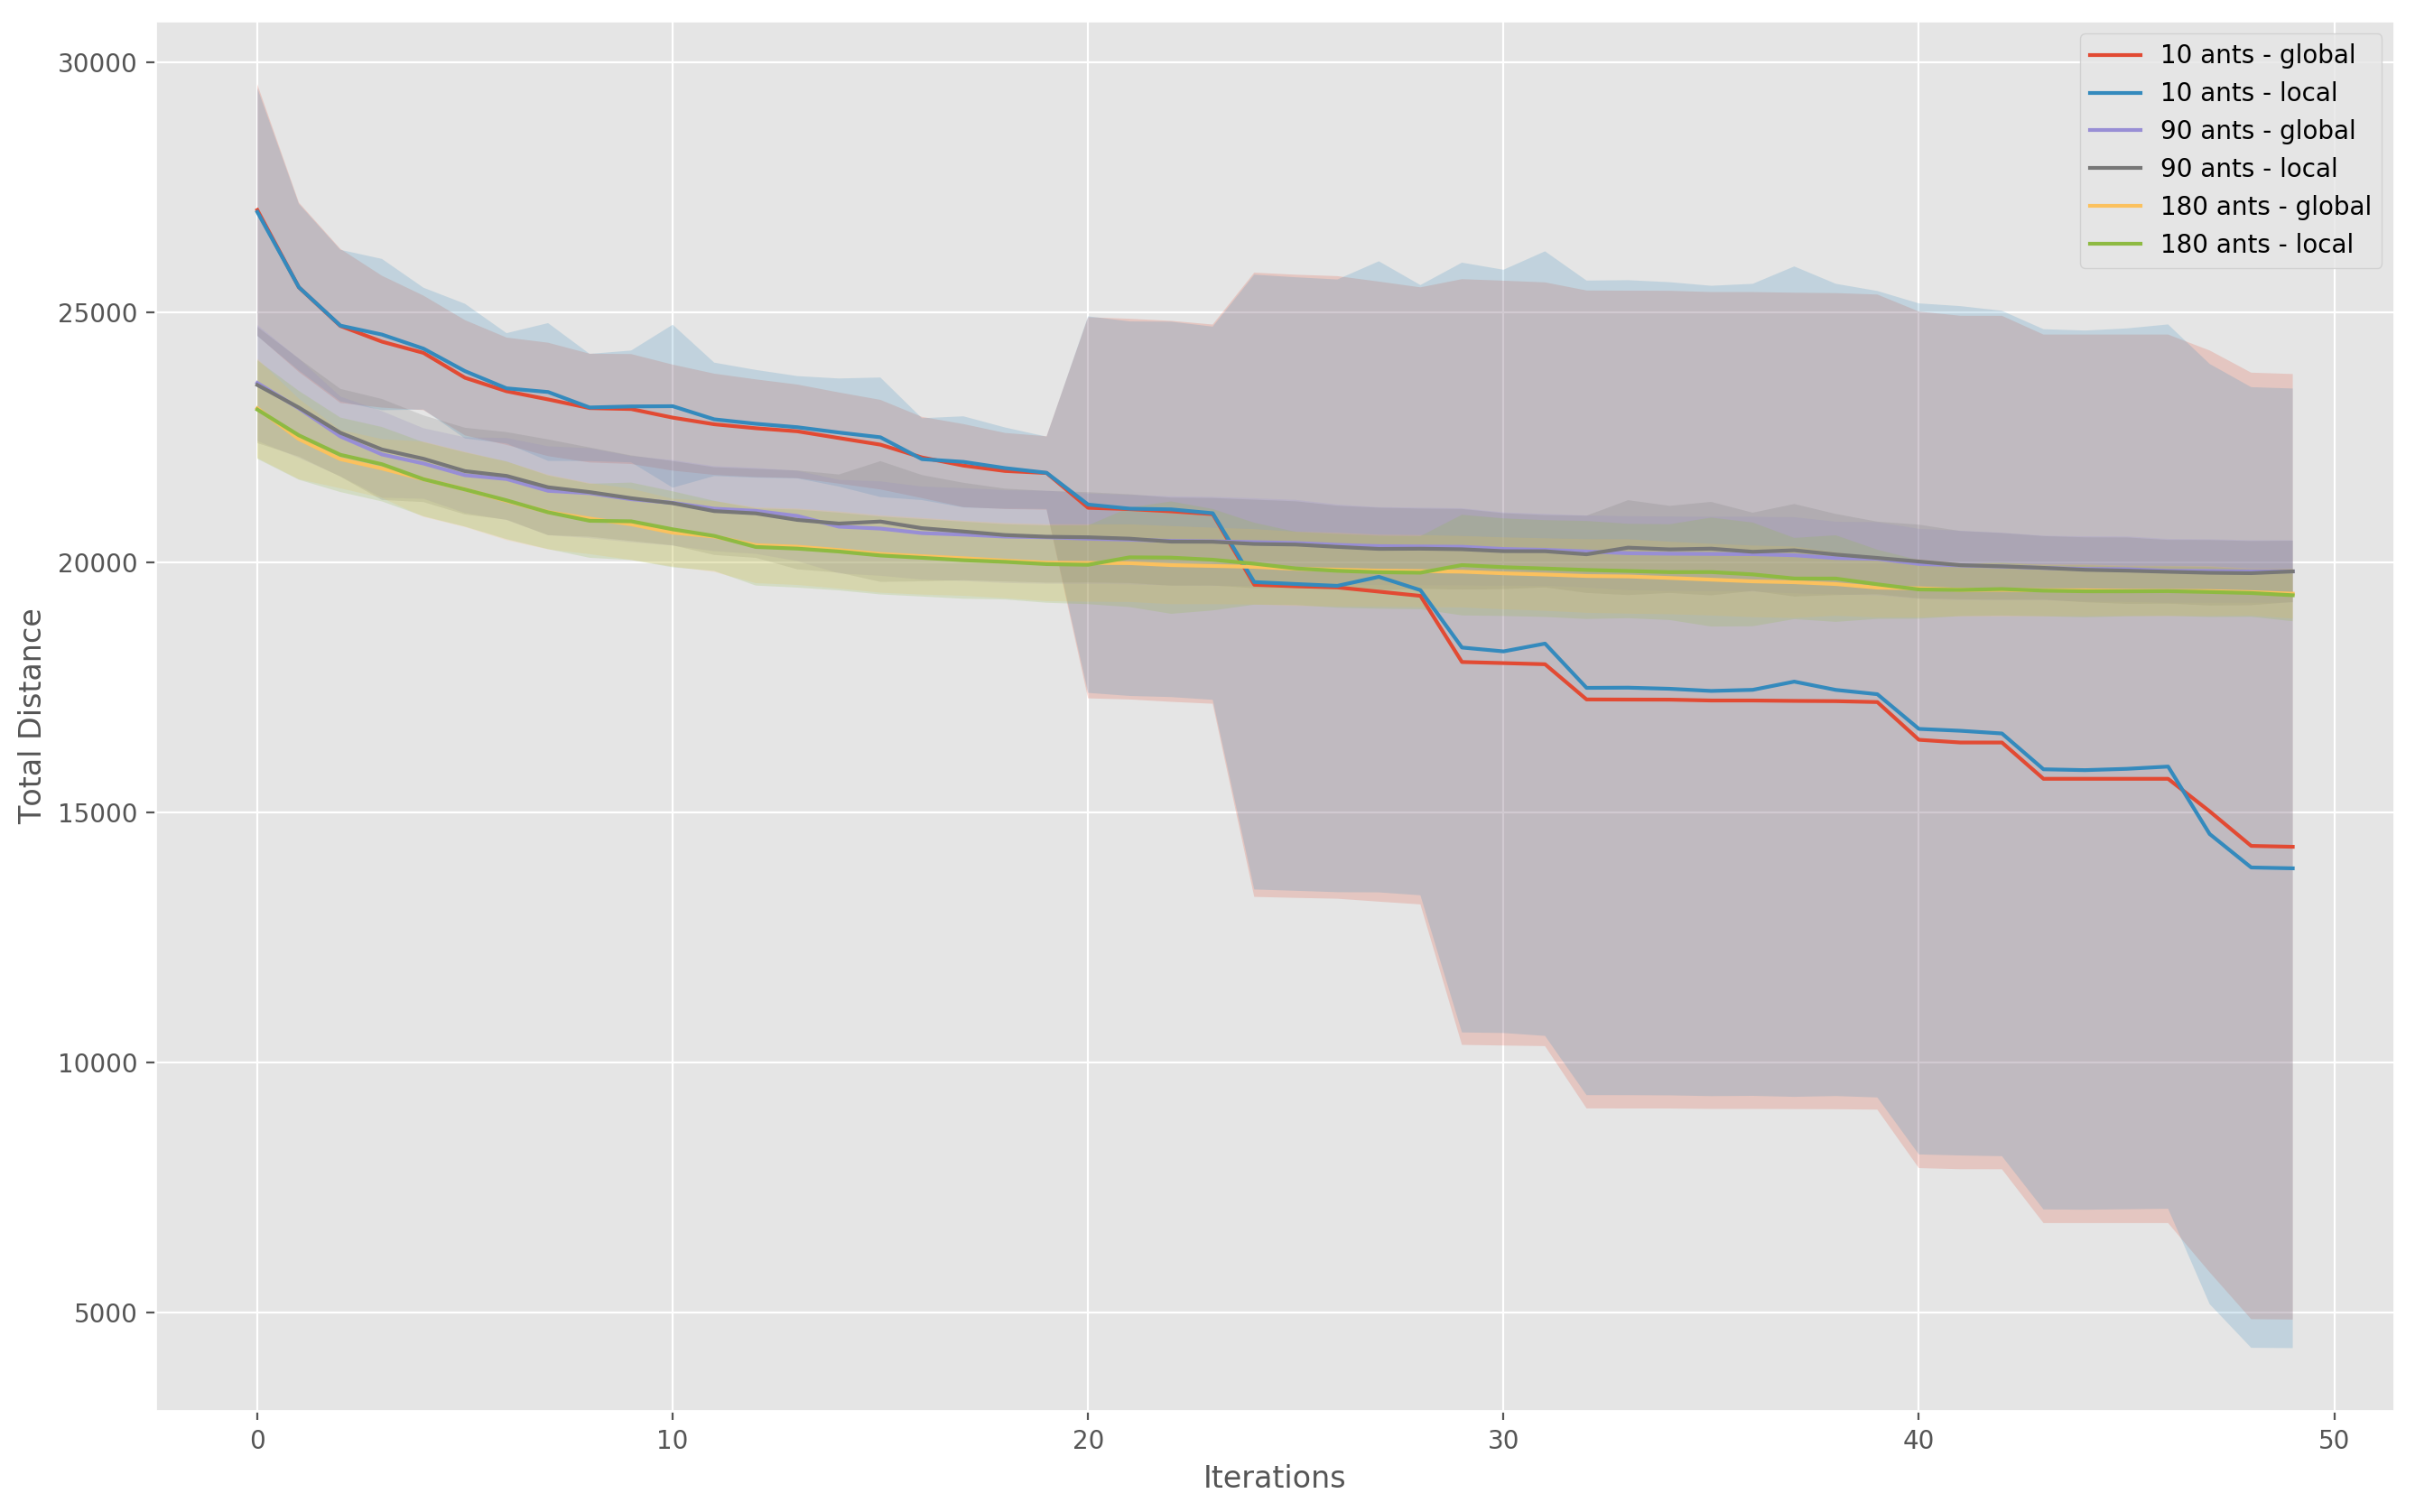
\includegraphics[width=11cm,keepaspectratio]{images/SJC1_ants.png}
  \caption{Média e desvio padrão para a distância da solução encontrada para base SJC1 com número de formigas variável.}
  \label{fig:sjc1_ants}
\end{figure}

Em seguida avaliamos os efeitos da variação da taxa de evaporação do feromônio($\rho$). Na Figura \ref{fig:sjc1_rho} vemos algo peculiar: os valores 0, 0.1 e 0.5 para a $\rho$ se sobrepõem no gráfico, pois geram exatamente os mesmos resultados. Como a evaporação do feromônio é muito sutil, o que provavelmente acontece é que o resultado do termo $\rho(\Delta\tau_i - \tau_i)$ fica muito pequeno a ponto de se tornar irrelevante para levar as soluções para outro caminho, ou seja, o espaço de soluções é mal explorado. O melhor valor para $\rho$ encontrado foi \textbf{0.99}. Com $\rho \geq 1$ o algoritmo não consegue progredir.

\begin{figure}[h]	
  \centering
  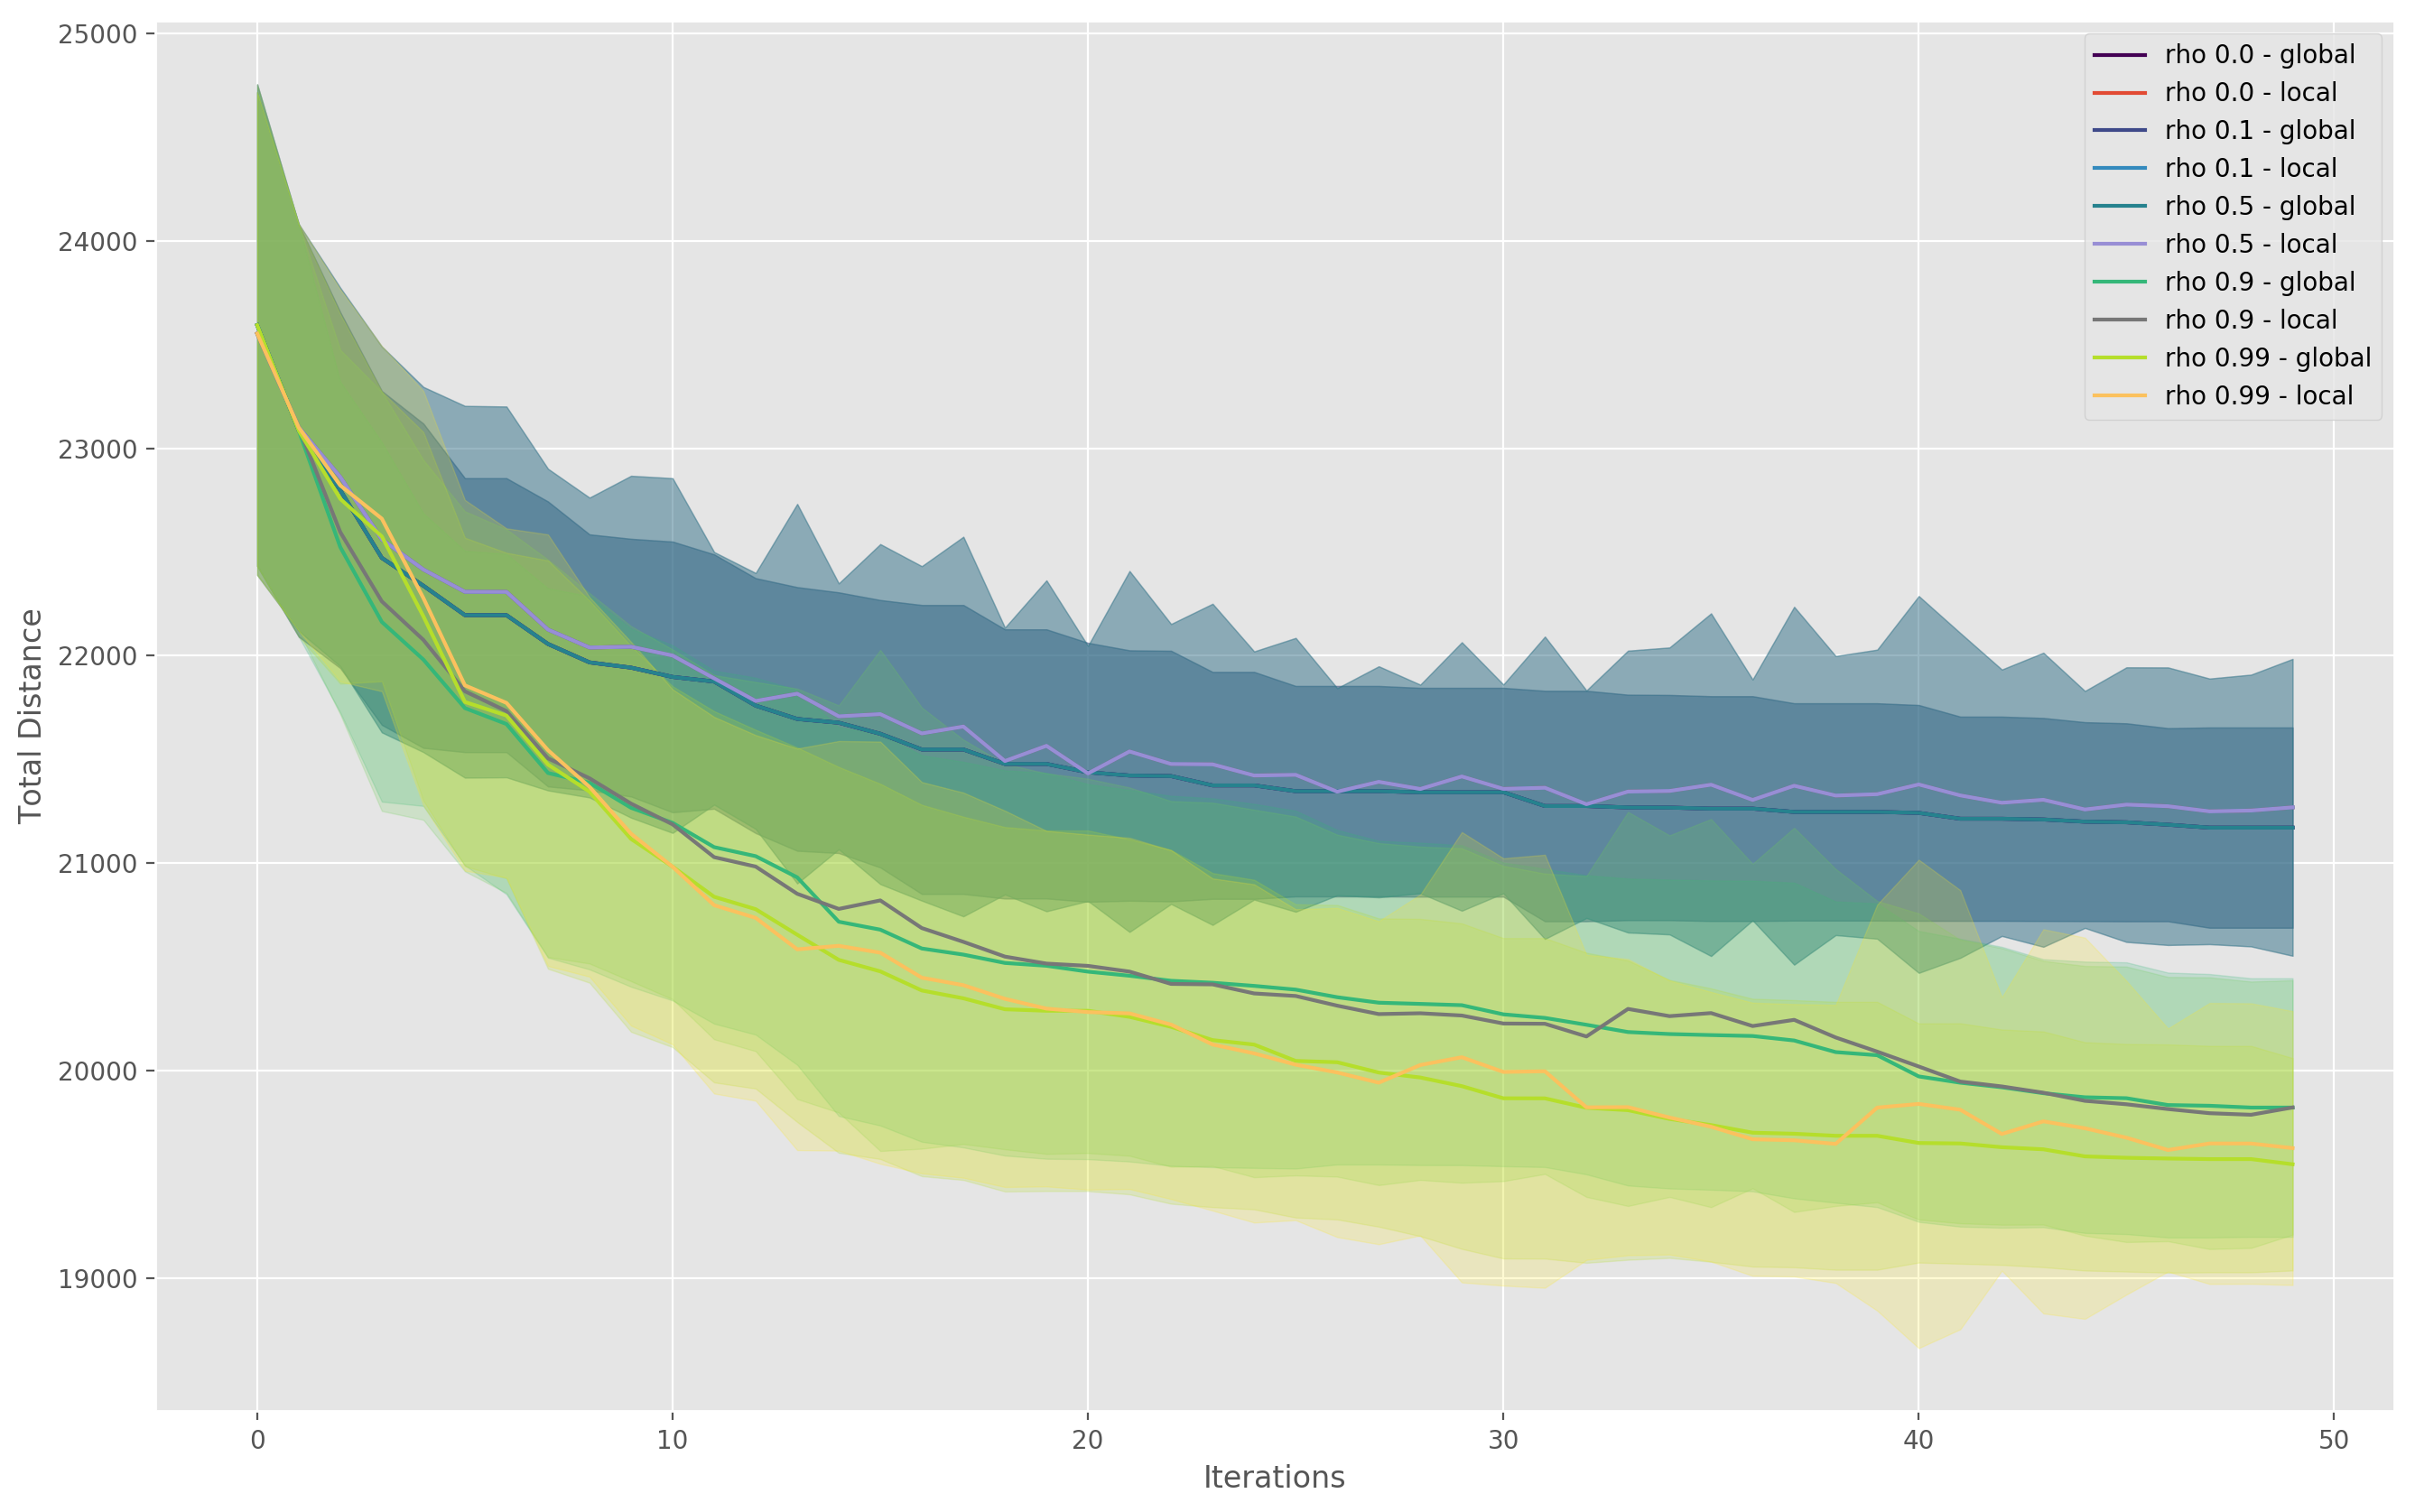
\includegraphics[width=11cm,keepaspectratio]{images/SJC1_rho.png}
  \caption{Média e desvio padrão para a distância da solução encontrada para base SJC1 com taxa de evaporação de feromônio variável.}
  \label{fig:sjc1_rho}
\end{figure}

Como última variação vamos analisar a influência dos indicadores $\alpha$ e $\beta$. Pelo gráfico na Figura \ref{fig:sjc1_alpha_beta} podemos ver que, apesar de a média do melhor global para $\alpha = 3$ e $\beta = 1$ ser melhor que a média do melhor local para $\alpha = 1$ e $\beta = 0$, a média global do último é melhor, o que contra o padrão dos resultados de \cite{de2005max}.

\begin{figure}[h]	
  \centering
  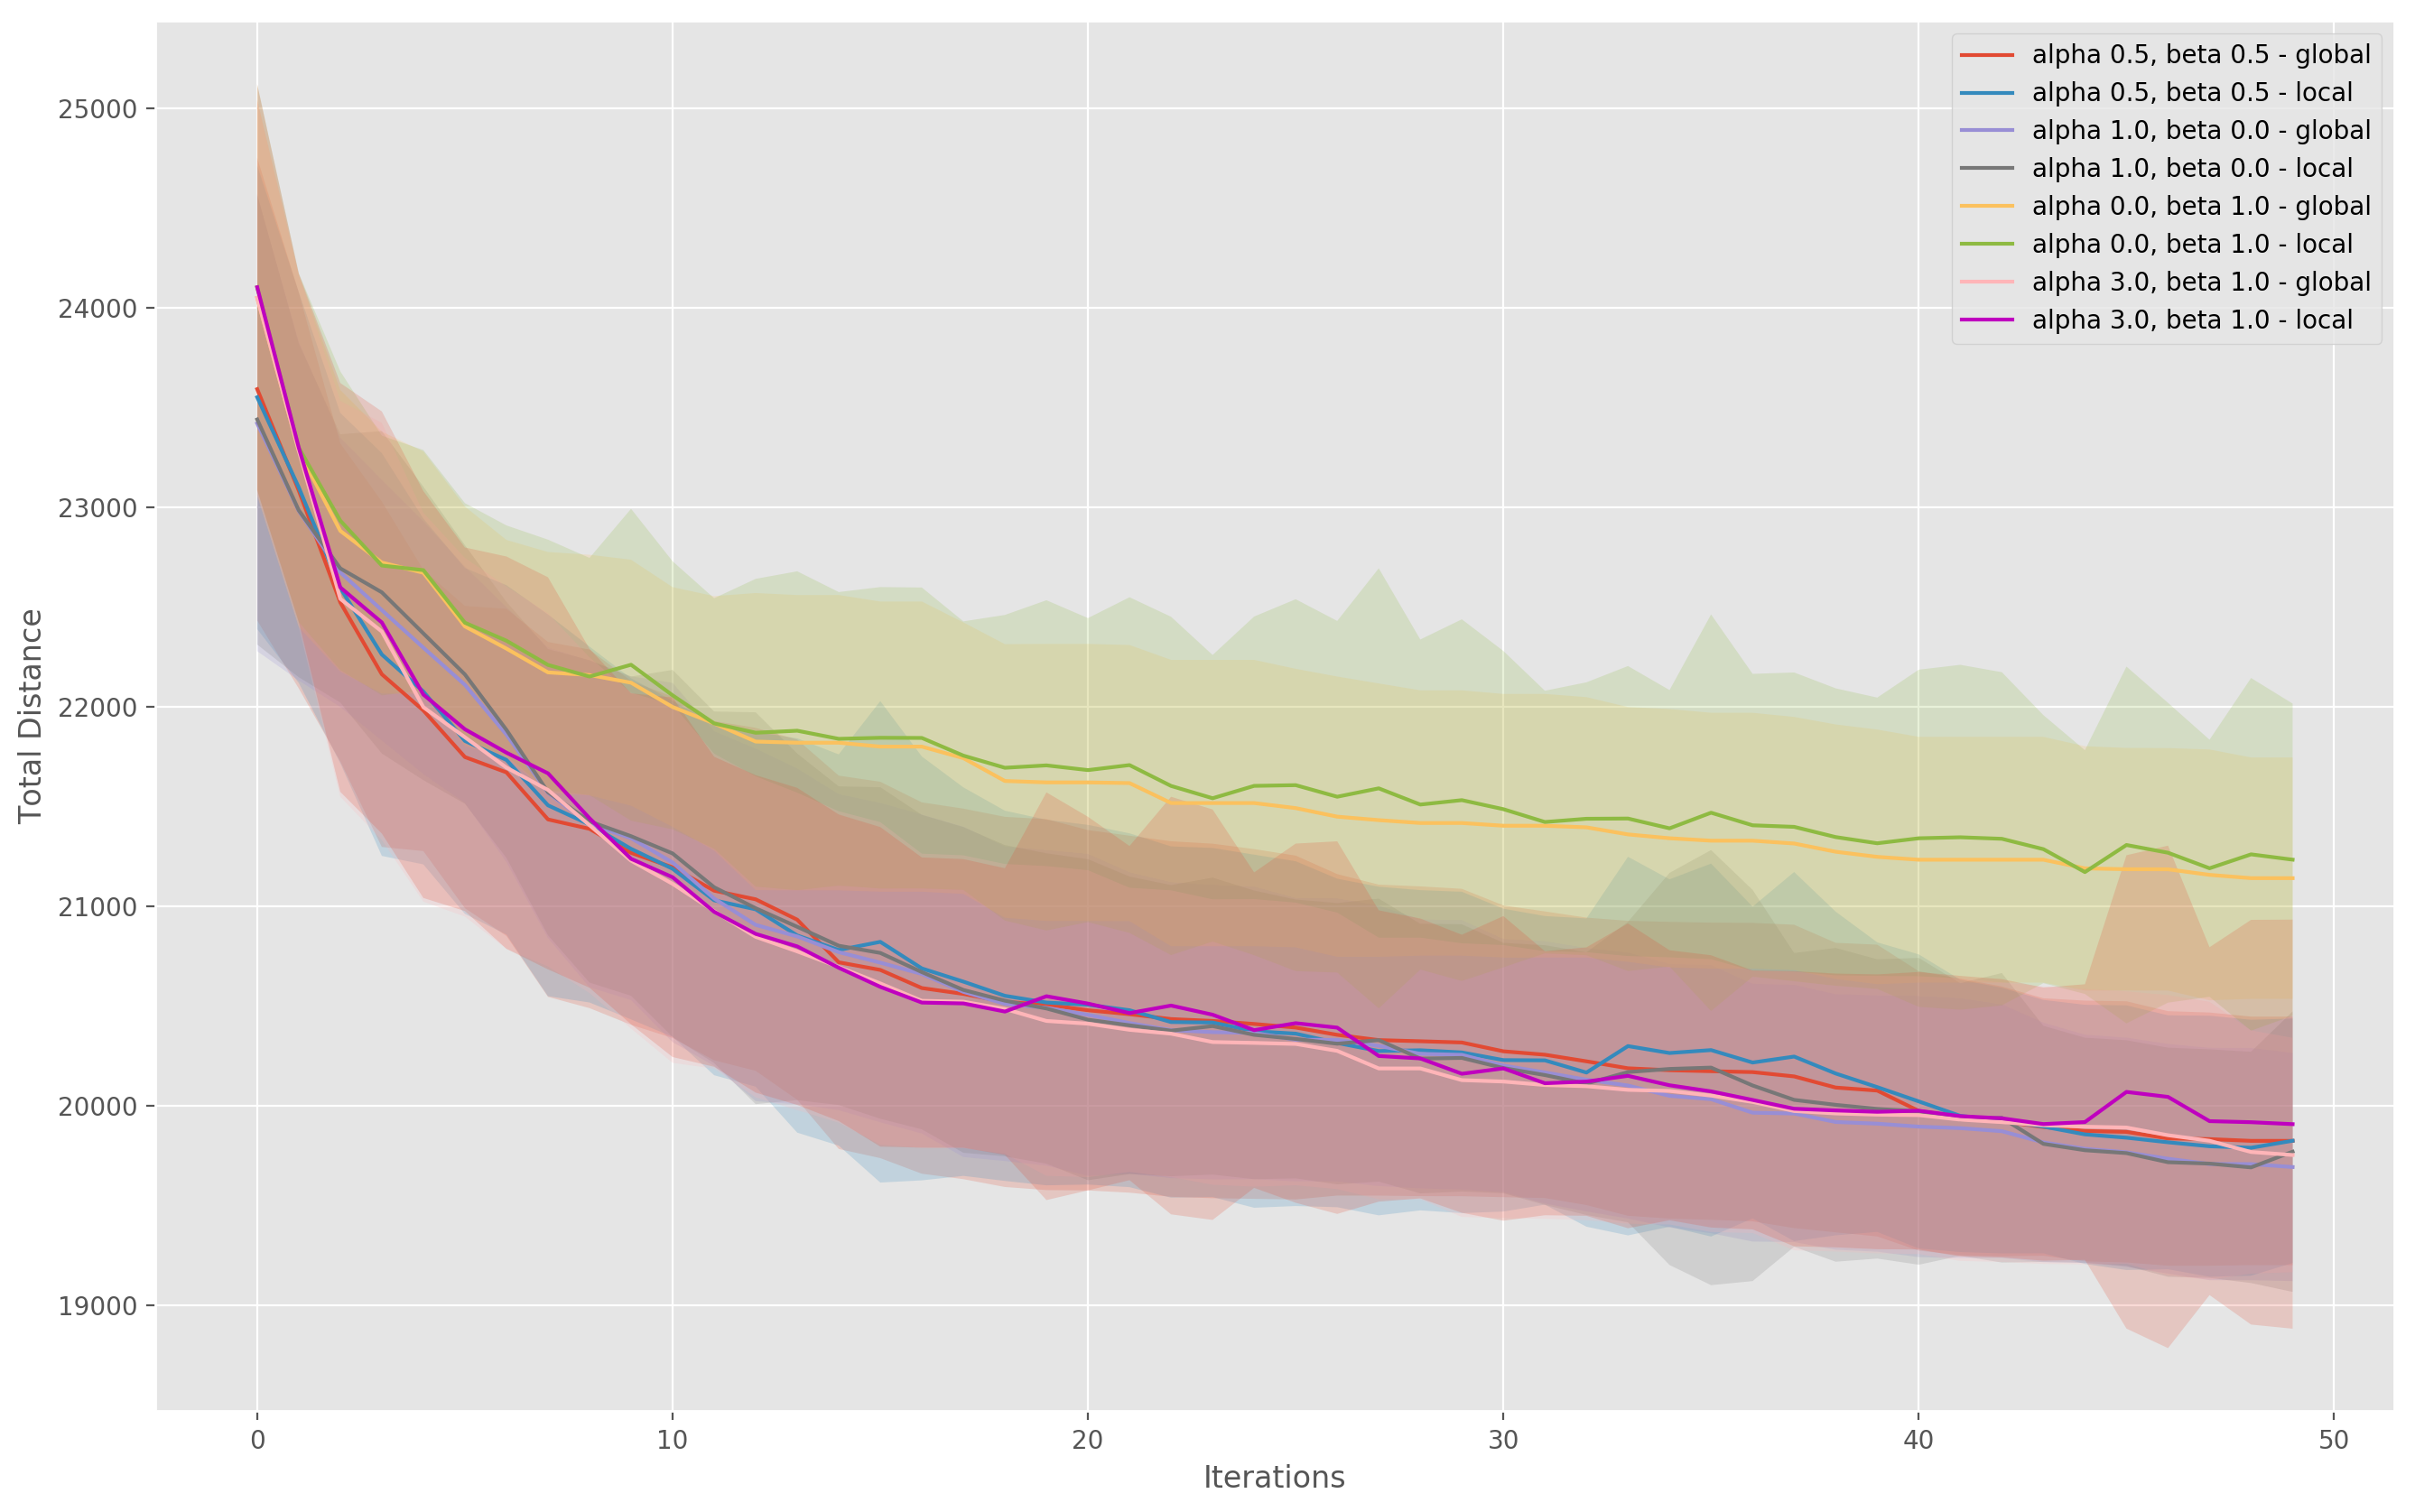
\includegraphics[width=11cm,keepaspectratio]{images/SJC1_alpha_beta.png}
  \caption{Média e desvio padrão para a distância da solução encontrada para base SJC1 com a variação dos pesos dos feromônios e da heurística de informação no cálculo da probabilidade de escolha do nó.}
  \label{fig:sjc1_alpha_beta}
\end{figure}

Por fim mostramos na Figura \ref{fig:sjc1_best} o melhor resultado encontrado entre as repetições para todas as variações de parâmetros testadas até agora. A melhor combinação de parâmetros foi 100 iterações, 180 formigas, $\rho = 0.99$, $\alpha=1$ e $\beta=0$ Ignorando a execução problemática, a combinação dos melhores parâmetros encontrados até agora foi a que performou melhor, alcançando, na melhor das repetições, uma distância total de \textbf{18009.965} entre os clientes e os centros. 

\begin{figure}[h]	
  \centering
  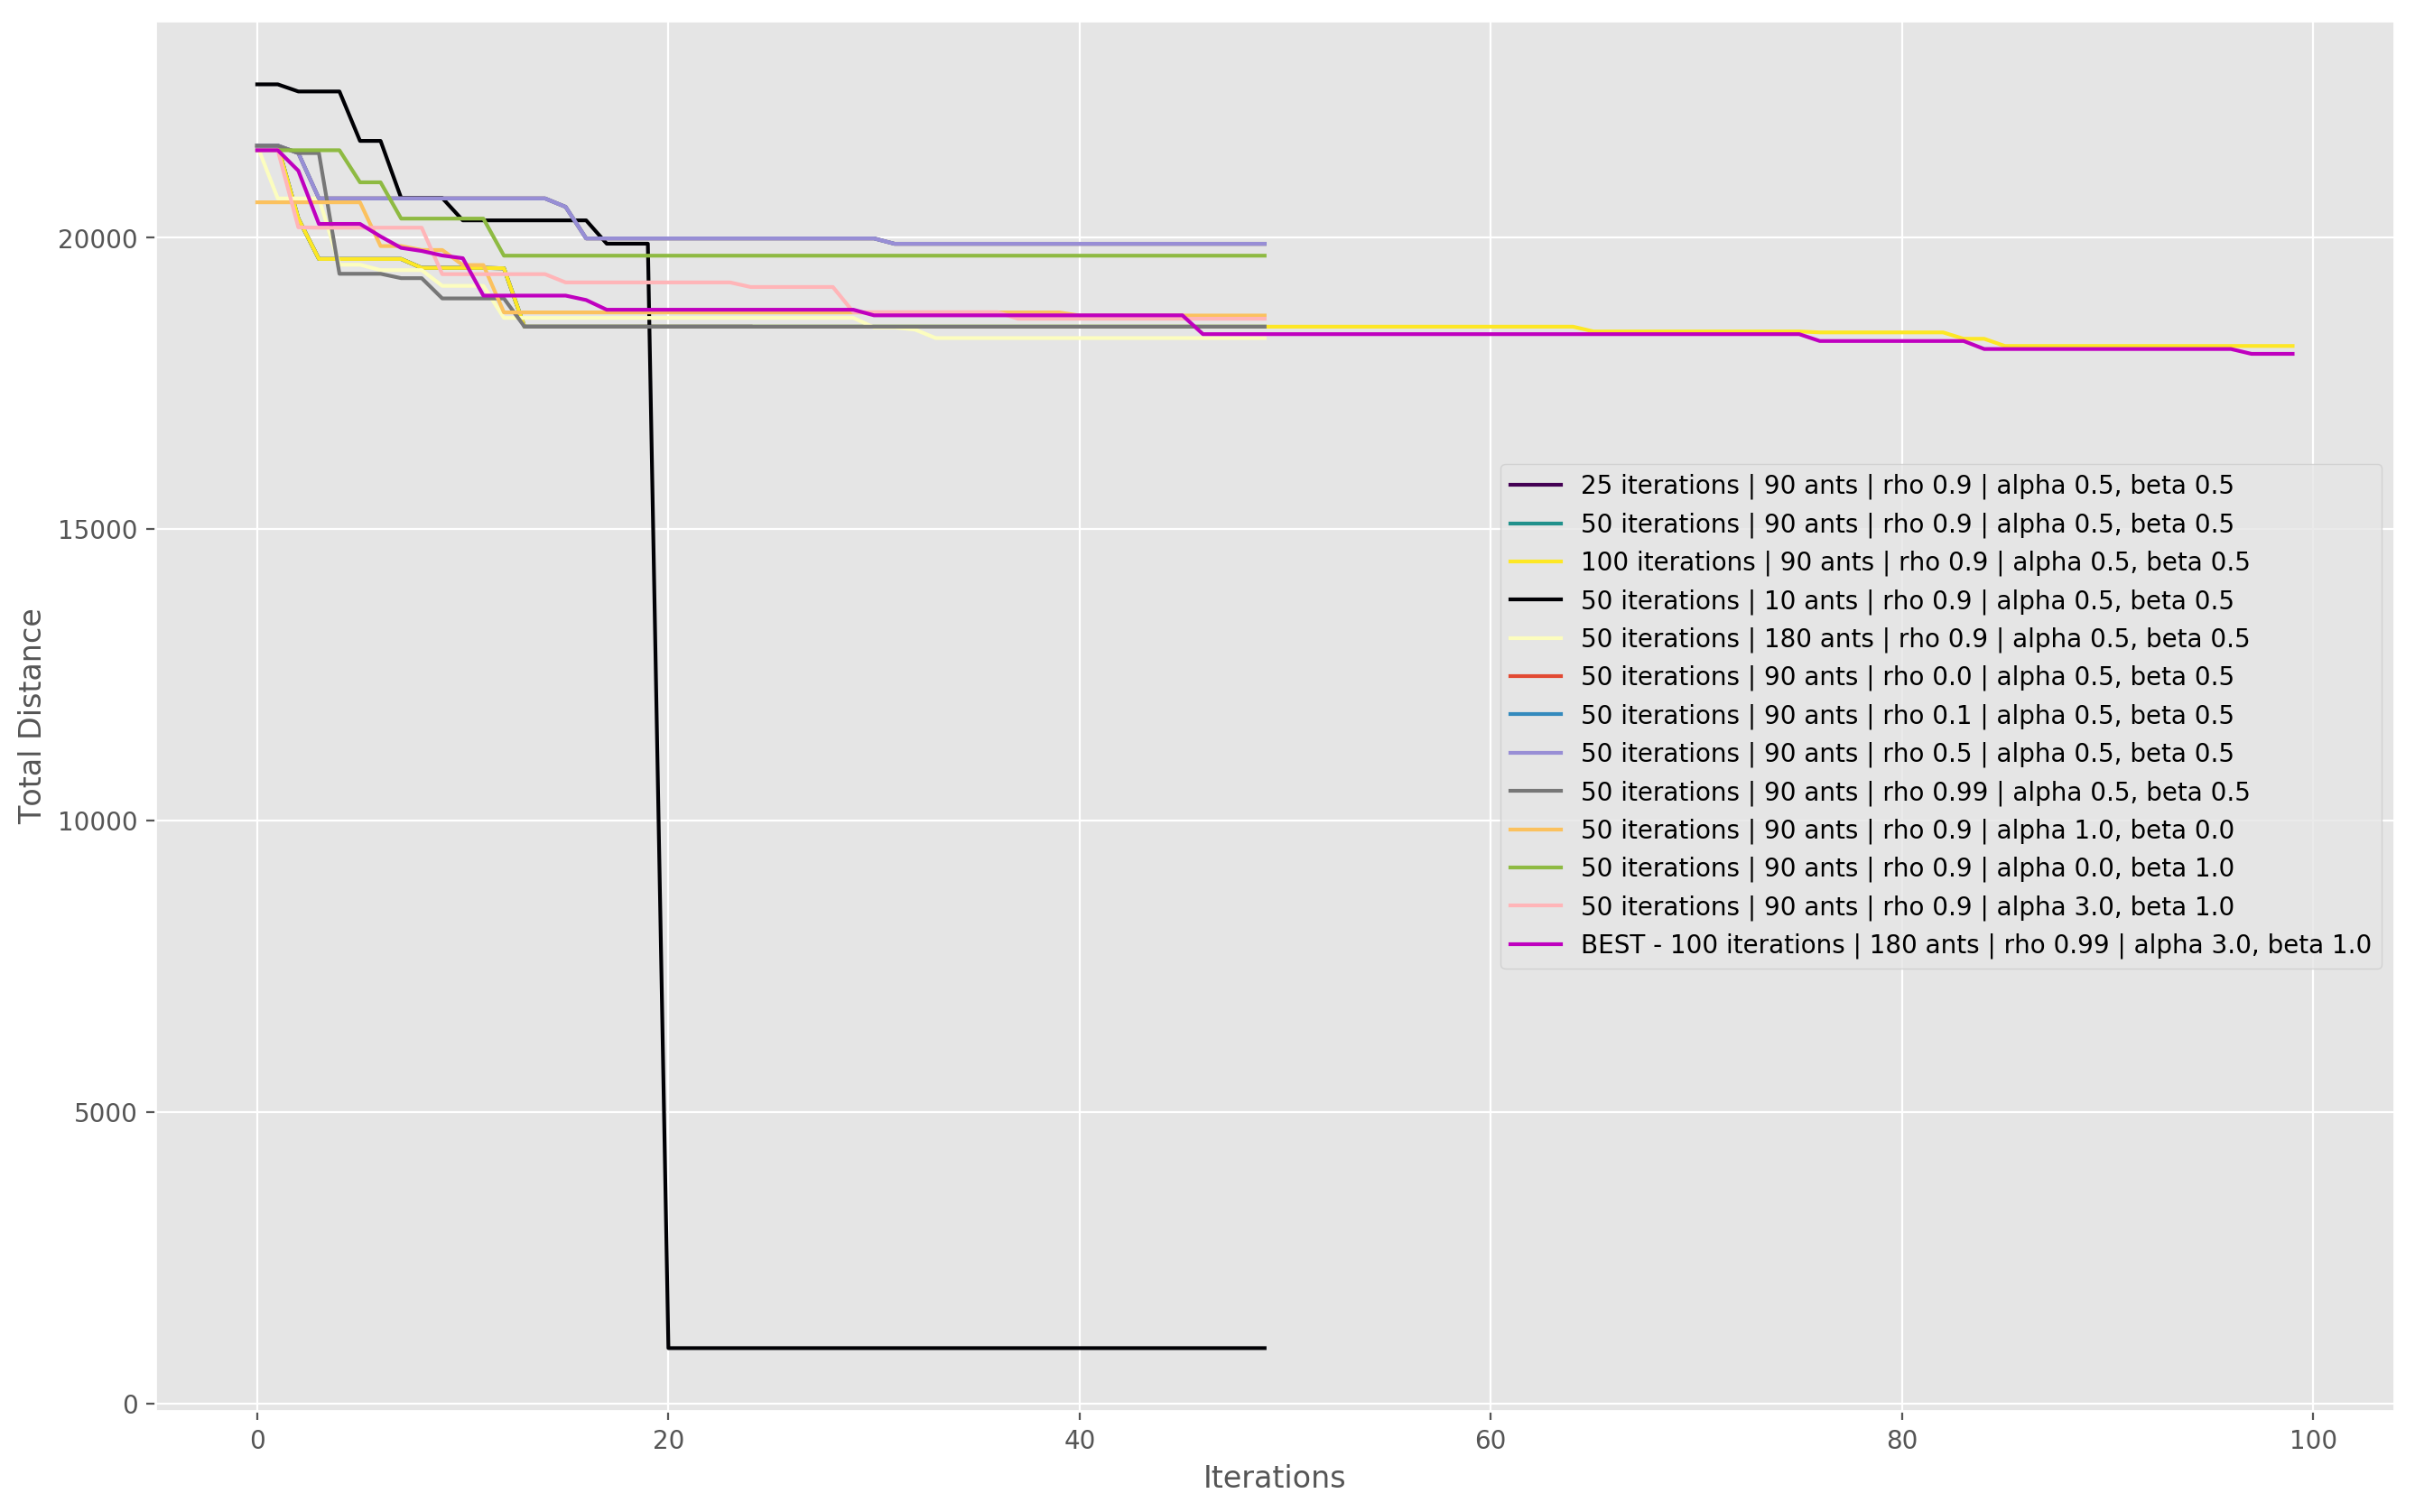
\includegraphics[width=11cm,keepaspectratio]{images/SJC1_best.png}
  \caption{Melhores soluções encontradas para a base SJC1 ao longo das repetições para todas as variações de parâmetros apresentadas até agora.}
  \label{fig:sjc1_best}
\end{figure}



\subsubsection{SJC2}

A base de dados SJC2 é composta de 200 pontos, todos com capacidade 840, mas com demanda variável. Ela busca por 15 pontos de mediana. Novamente vamos começar avaliando os resultados gerados para diferentes números de gerações. Em realidade, a análise experimental para essa base se dará com a mesma estrutura da base anterior, assim como ocorrerá com a base seguinte. Aqui, novamente o maior número de iterações se mostrou superior, como visto na Figura \ref{fig:sjc2_iterations}.

\begin{figure}[h]	
  \centering
  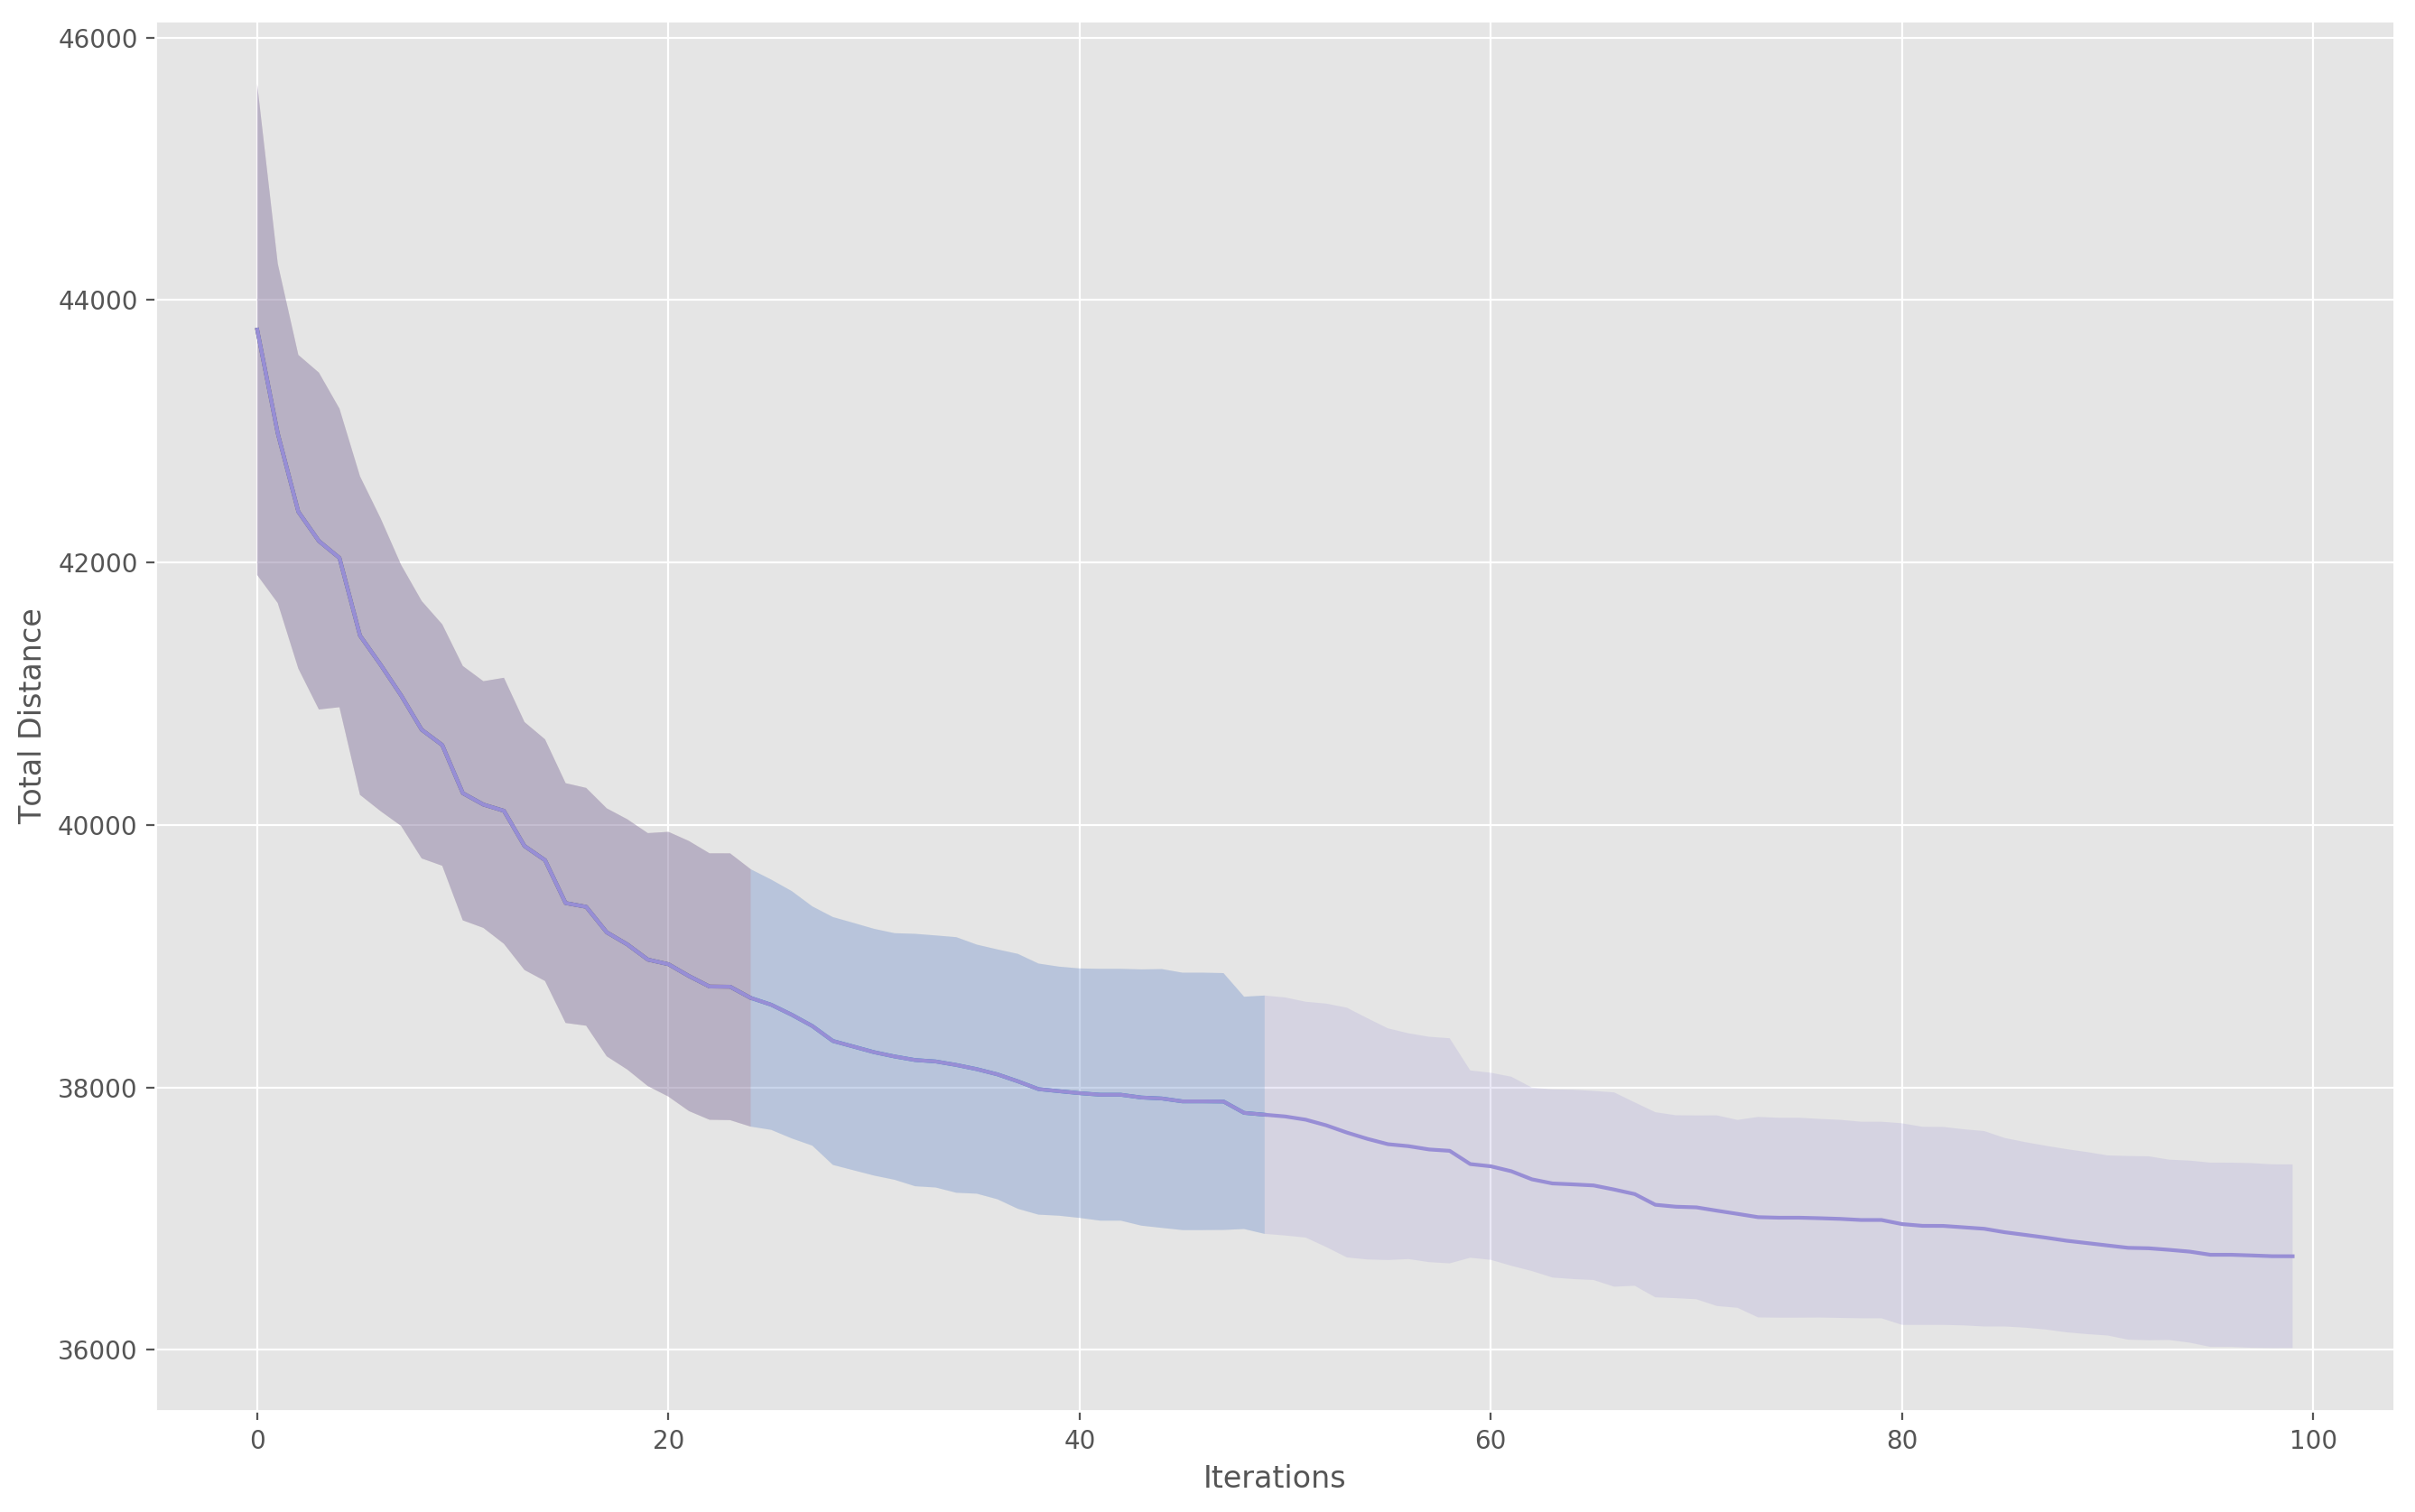
\includegraphics[width=11cm,keepaspectratio]{images/SJC2_iterations.png}
  \caption{Média e desvio padrão para a distância da solução encontrada para base SJC2 com número de iterações variável.}
  \label{fig:sjc2_iterations}
\end{figure}

Ao variarmos o número de formigas na colônia também encontramos resultados semelhantes à base SCJ1, com $2 * (n - p)$ formigas se mostrando mais eficiente. Os resultados estão na Figura \ref{fig:sjc2_ants}.

\begin{figure}[h]	
  \centering
  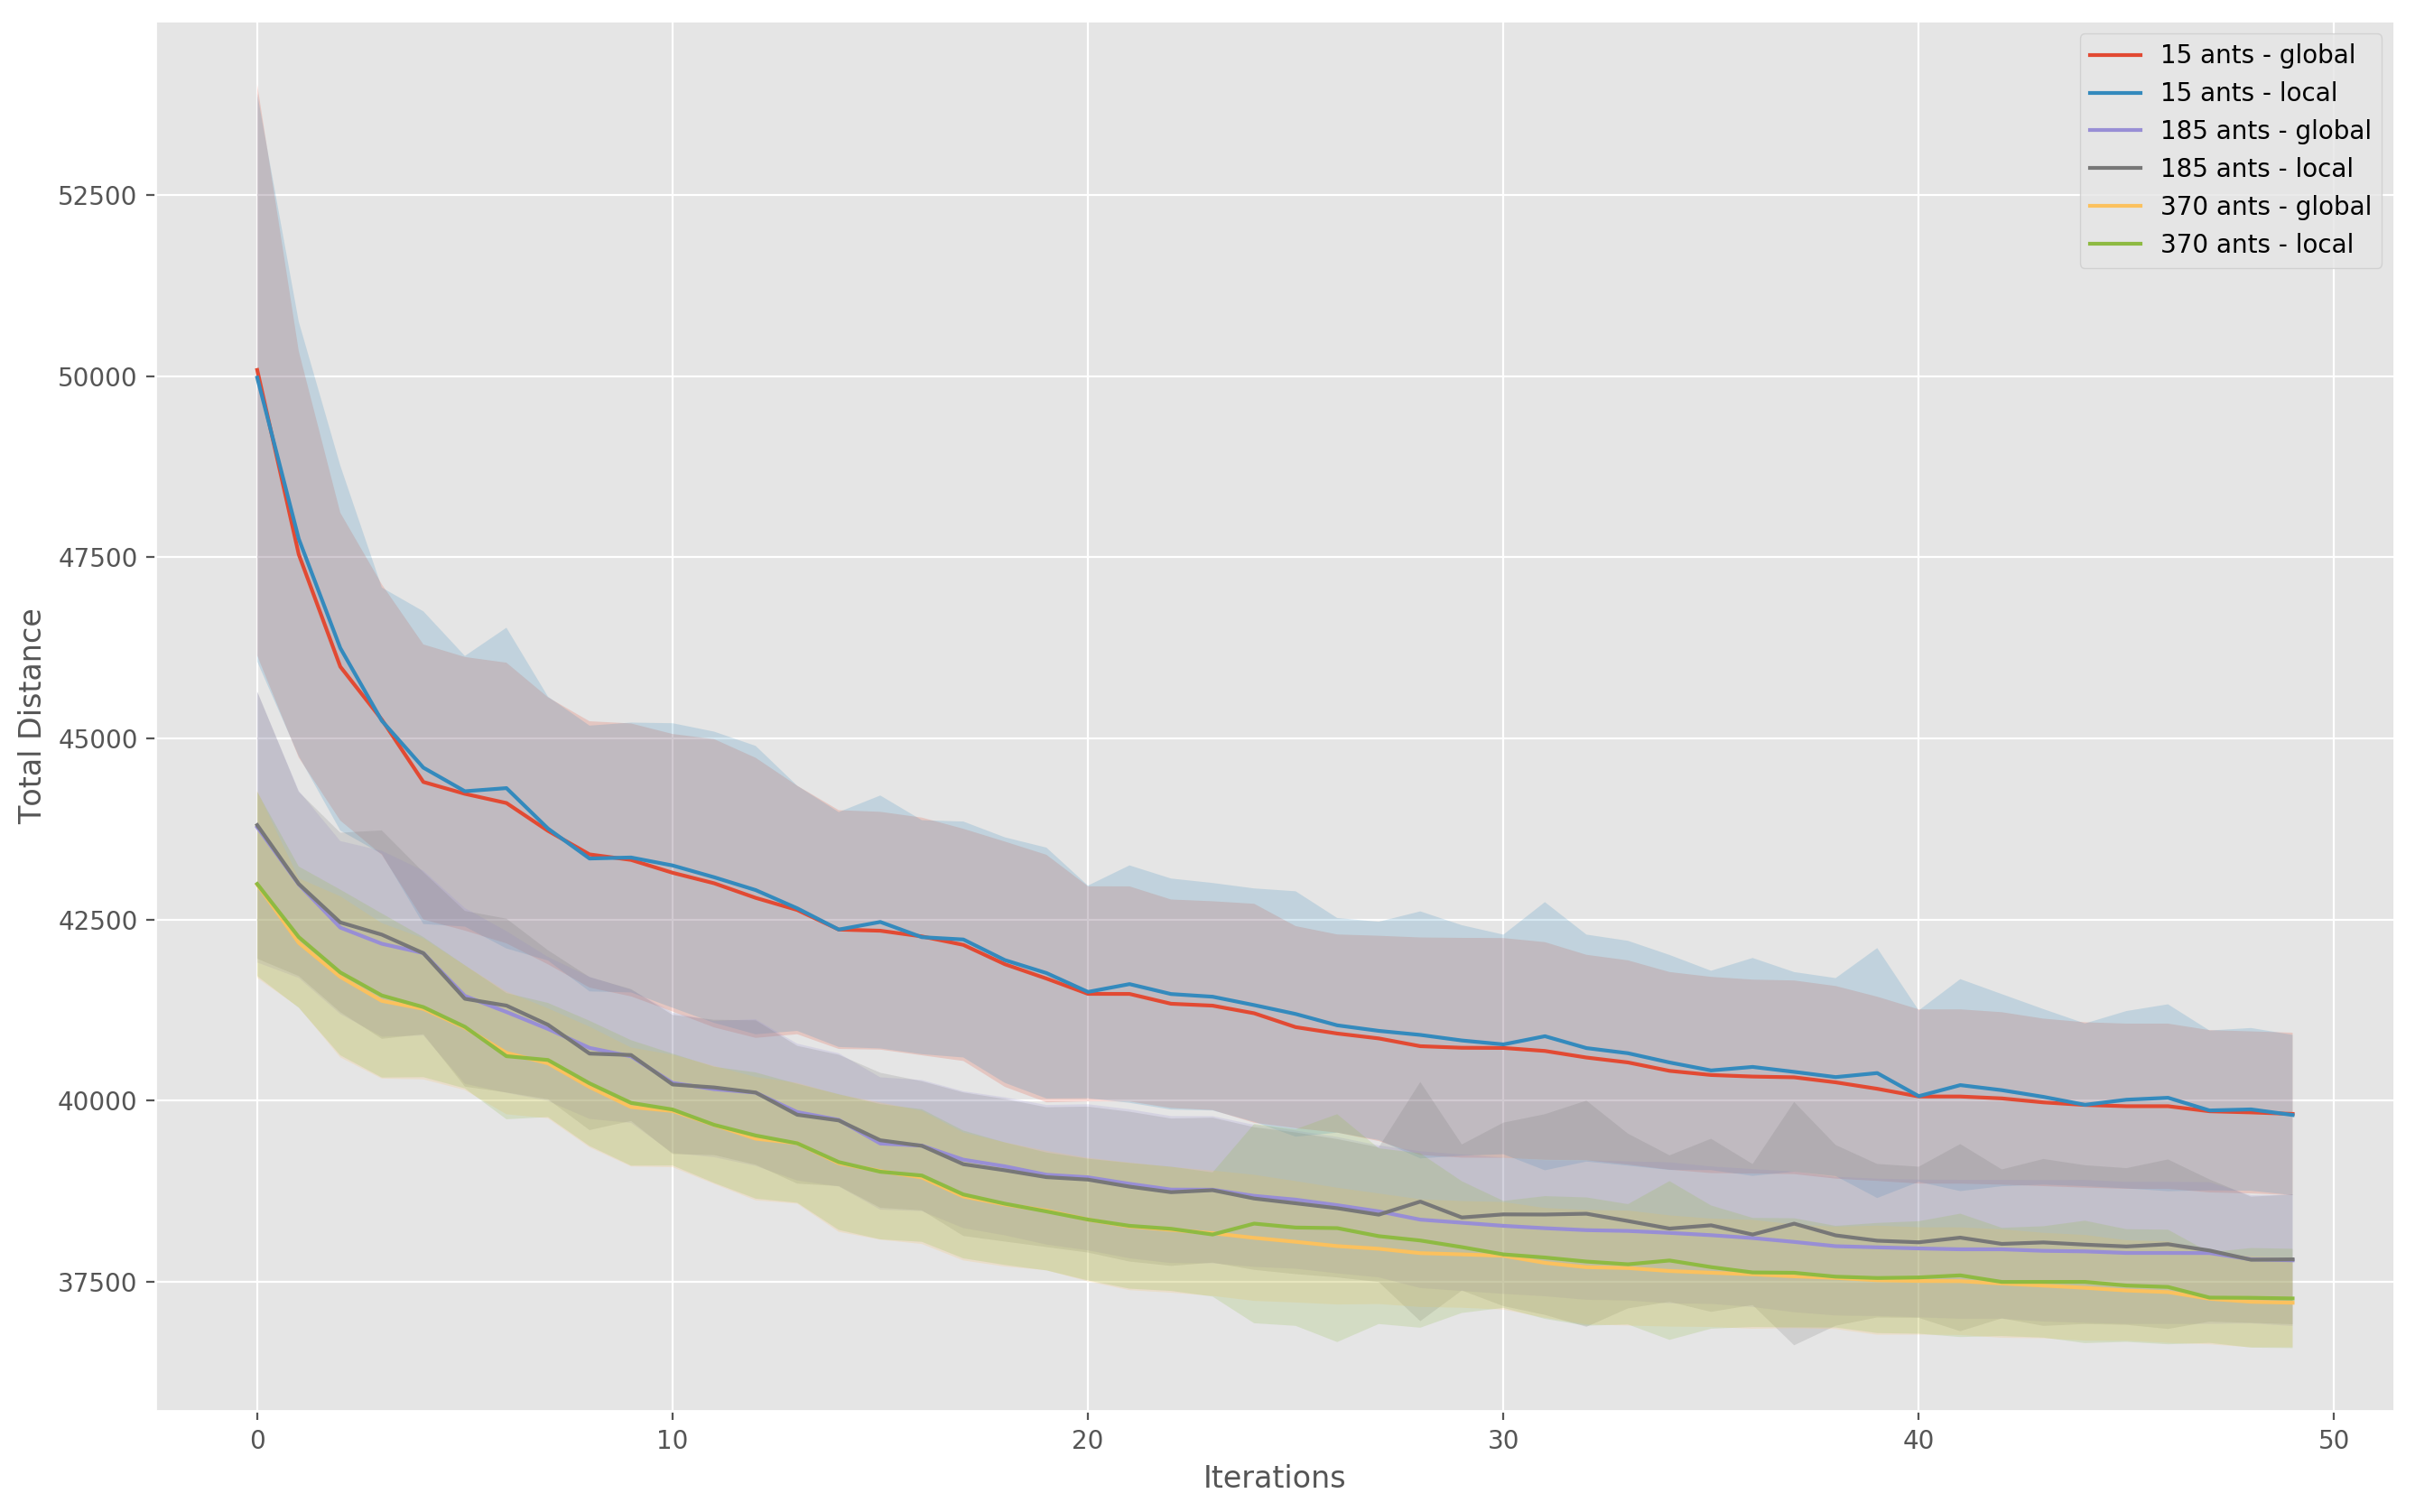
\includegraphics[width=11cm,keepaspectratio]{images/SJC2_ants.png}
  \caption{Média e desvio padrão para a distância da solução encontrada para base SJC2 com número de formigas variável.}
  \label{fig:sjc2_ants}
\end{figure}

Com relação ao termo $\rho$ encontramos um cenário idêntico ao da base anterior, como é possível ver na Figura \ref{fig:sjc2_rho}, ou seja, o valor ótimo é $\rho = 0.99$. 

\begin{figure}[h]	
  \centering
  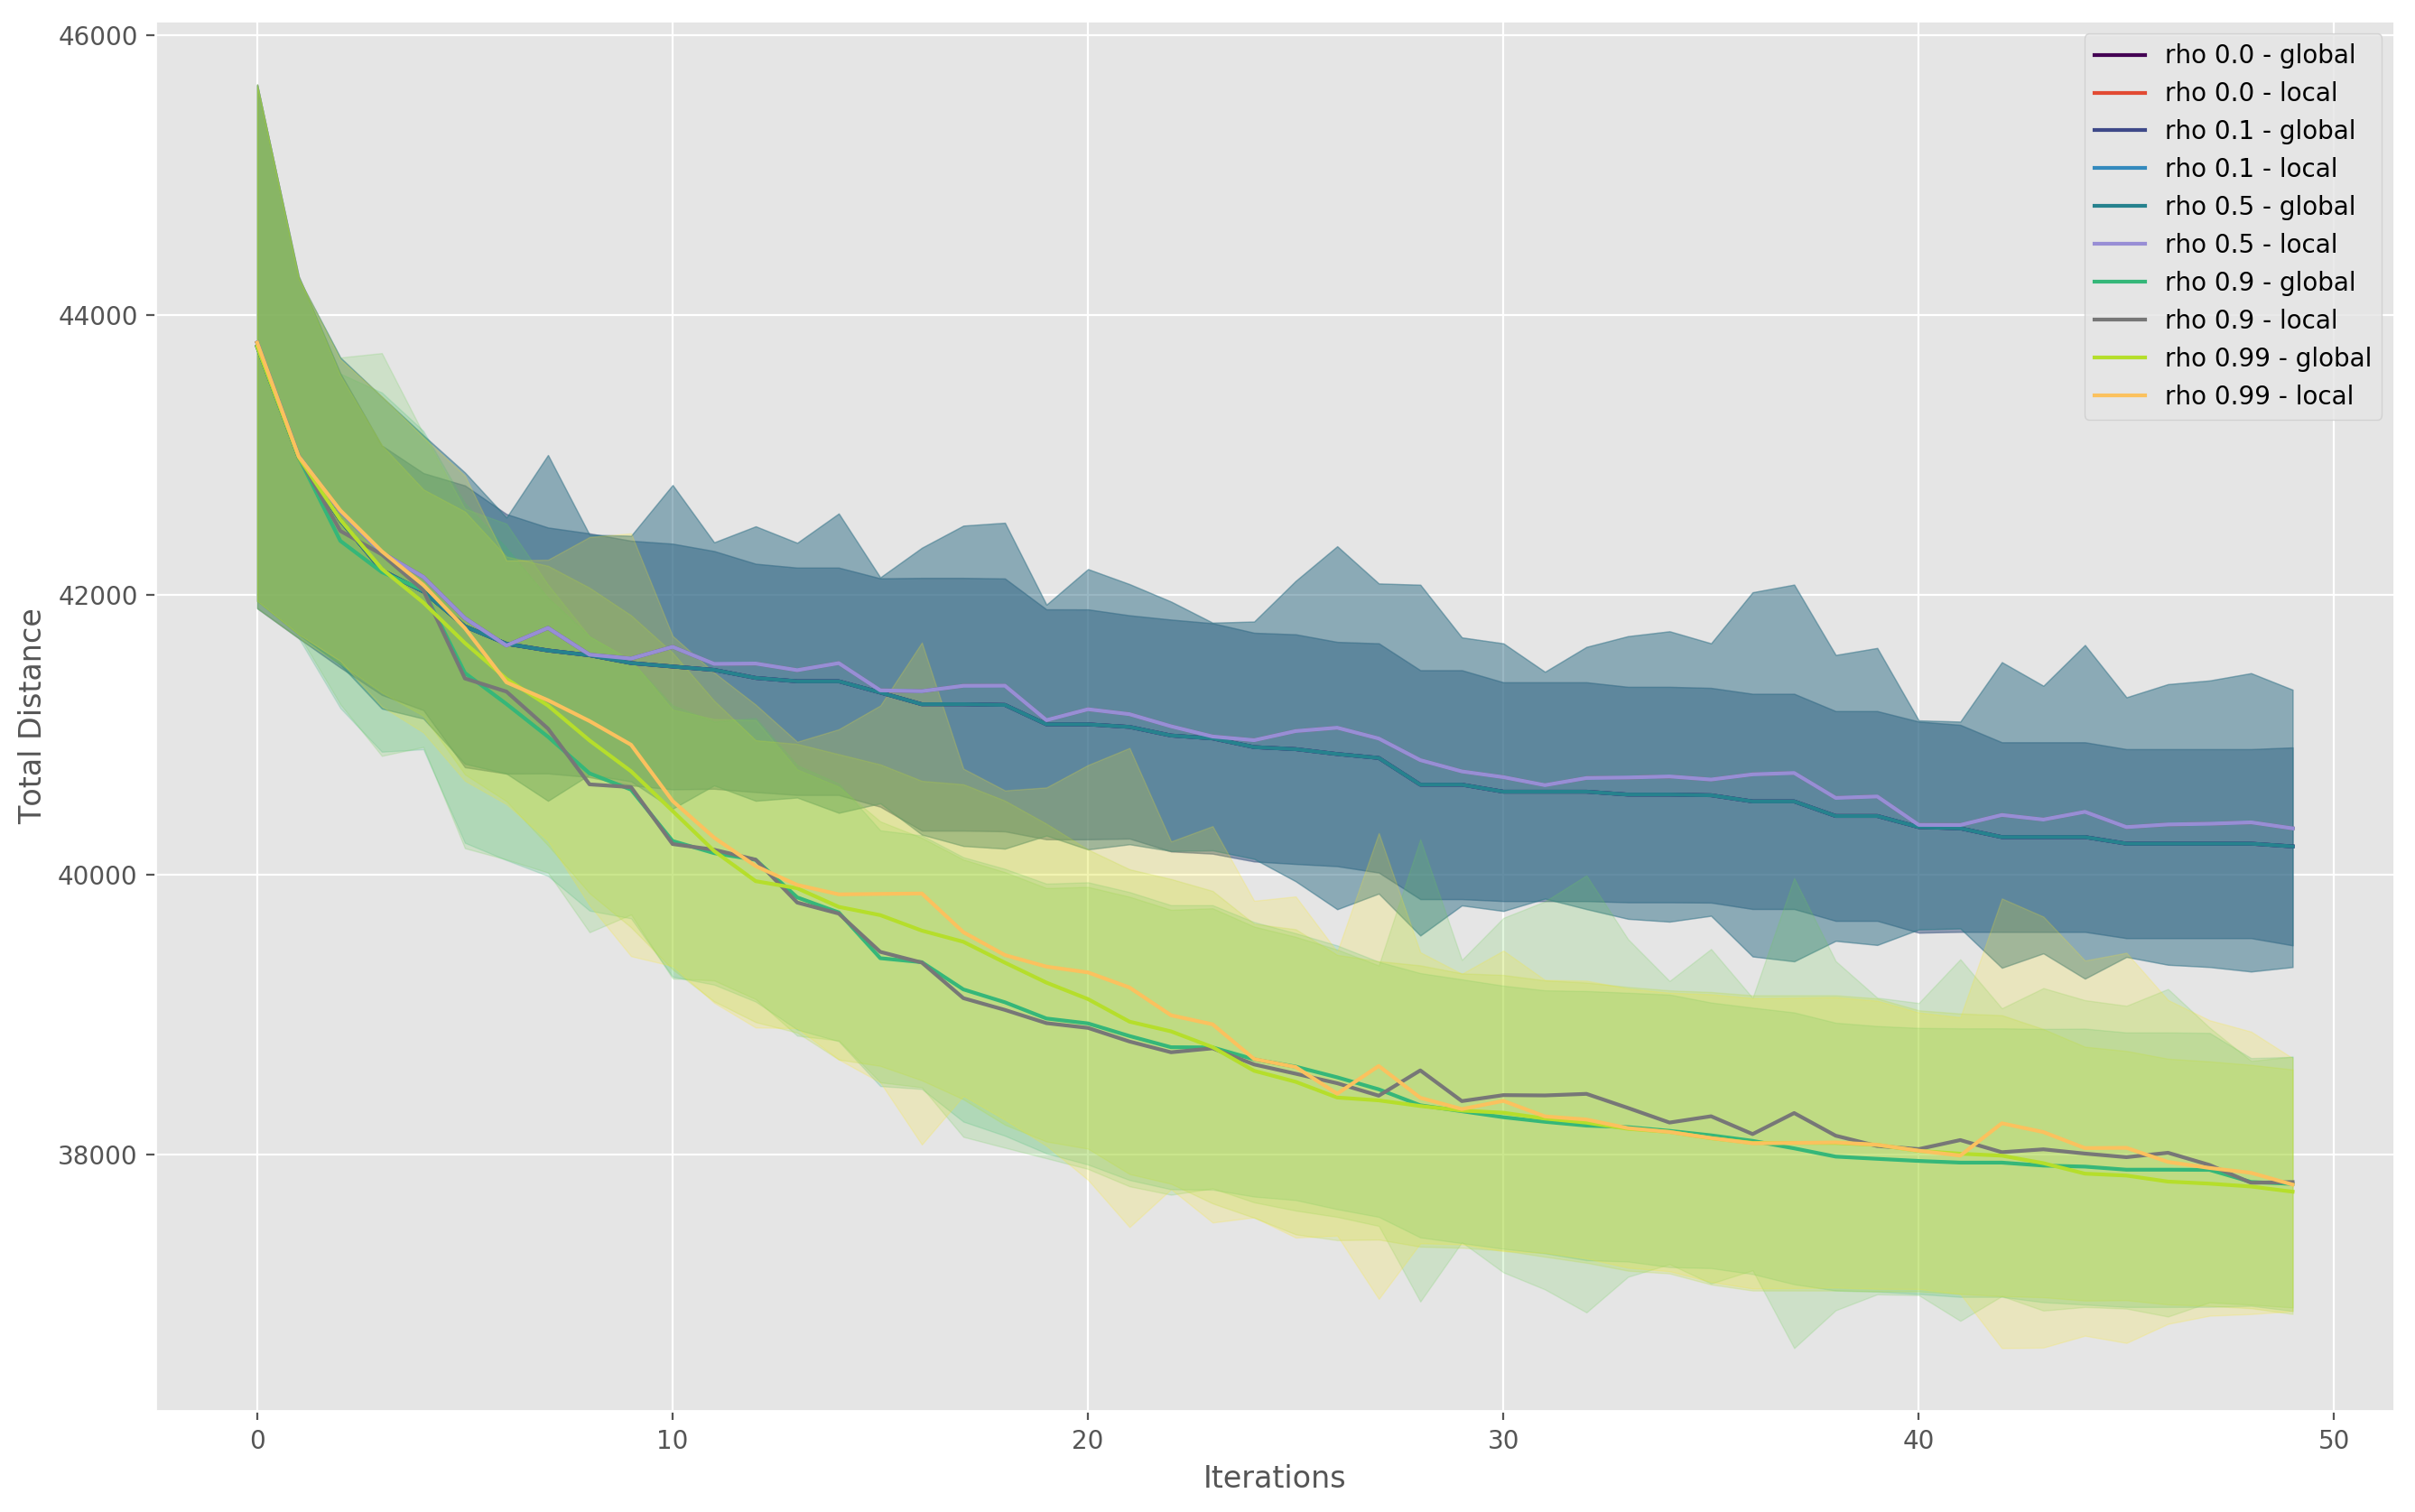
\includegraphics[width=11cm,keepaspectratio]{images/SJC2_rho.png}
  \caption{Média e desvio padrão para a distância da solução encontrada para base SJC2 com taxa de evaporação de feromônio variável.}
  \label{fig:sjc2_rho}
\end{figure}

Para os termos $\alpha$ e $\beta$ temos um resultado semelhante ao anterior: os valores ótimos são indubitavelmente $\alpha=1$ e $\beta=0$, o que vai novamente contra os resultados em \cite{de2005max}.

\begin{figure}[h]	
  \centering
  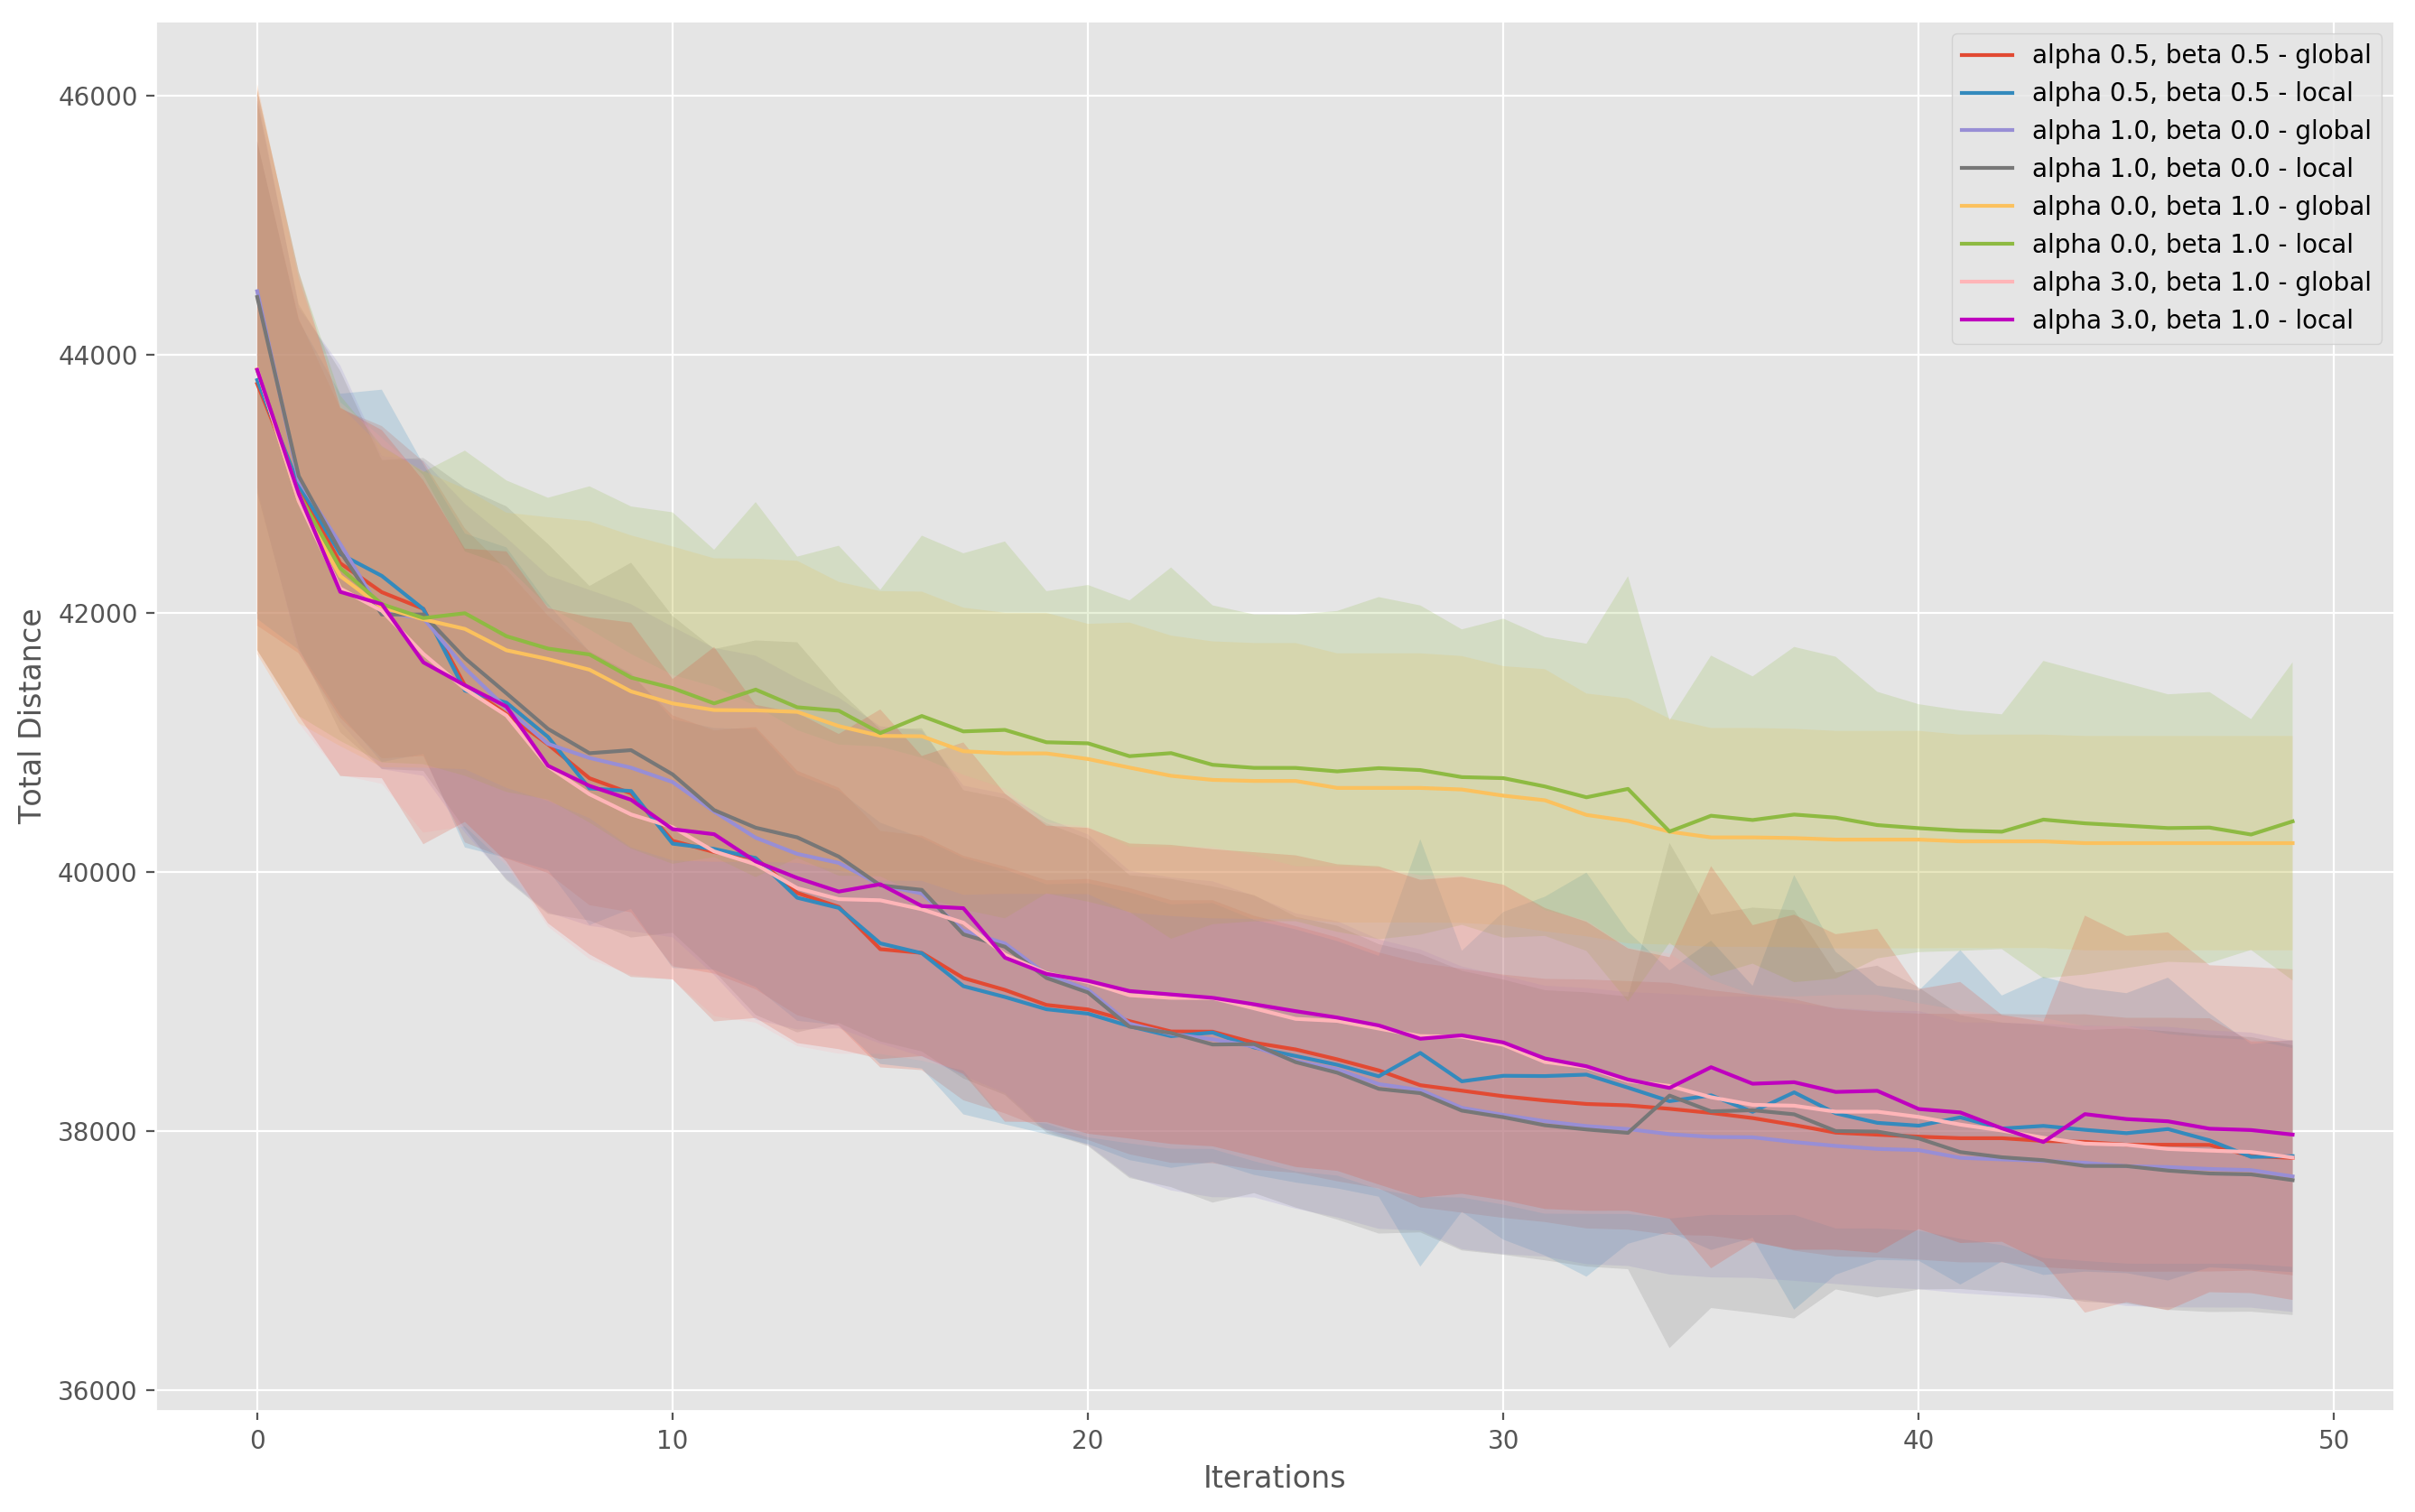
\includegraphics[width=11cm,keepaspectratio]{images/SJC2_alpha_beta.png}
  \caption{Média e desvio padrão para a distância da solução encontrada para base SJC2 com a variação dos pesos dos feromônios e da heurística de informação no cálculo da probabilidade de escolha do nó.}
  \label{fig:sjc2_alpha_beta}
\end{figure}

Juntos, os melhores parâmetros encontrados foram 100 iterações, 370 formigas, $\rho = 0.99$, $\alpha=1$ e $\beta=0$. Na Figura \ref{fig:sjc2_best} temos o gráfico dos melhores resultados para todas as variações de parâmetros. Surpreendentemente, conjunto dos melhores descrito acima não foi o que encontrou a melhor solução de todas, apesar de ter uma média melhor. O título ficou para a execução com 100 iterações, 185 formigas, $\rho = 0.9$, $\alpha=0.5$ e $\beta=0.5$, que encontrou uma solução de valor \textbf{35116.028} em uma de suas repetições.

\begin{figure}[h]	
  \centering
  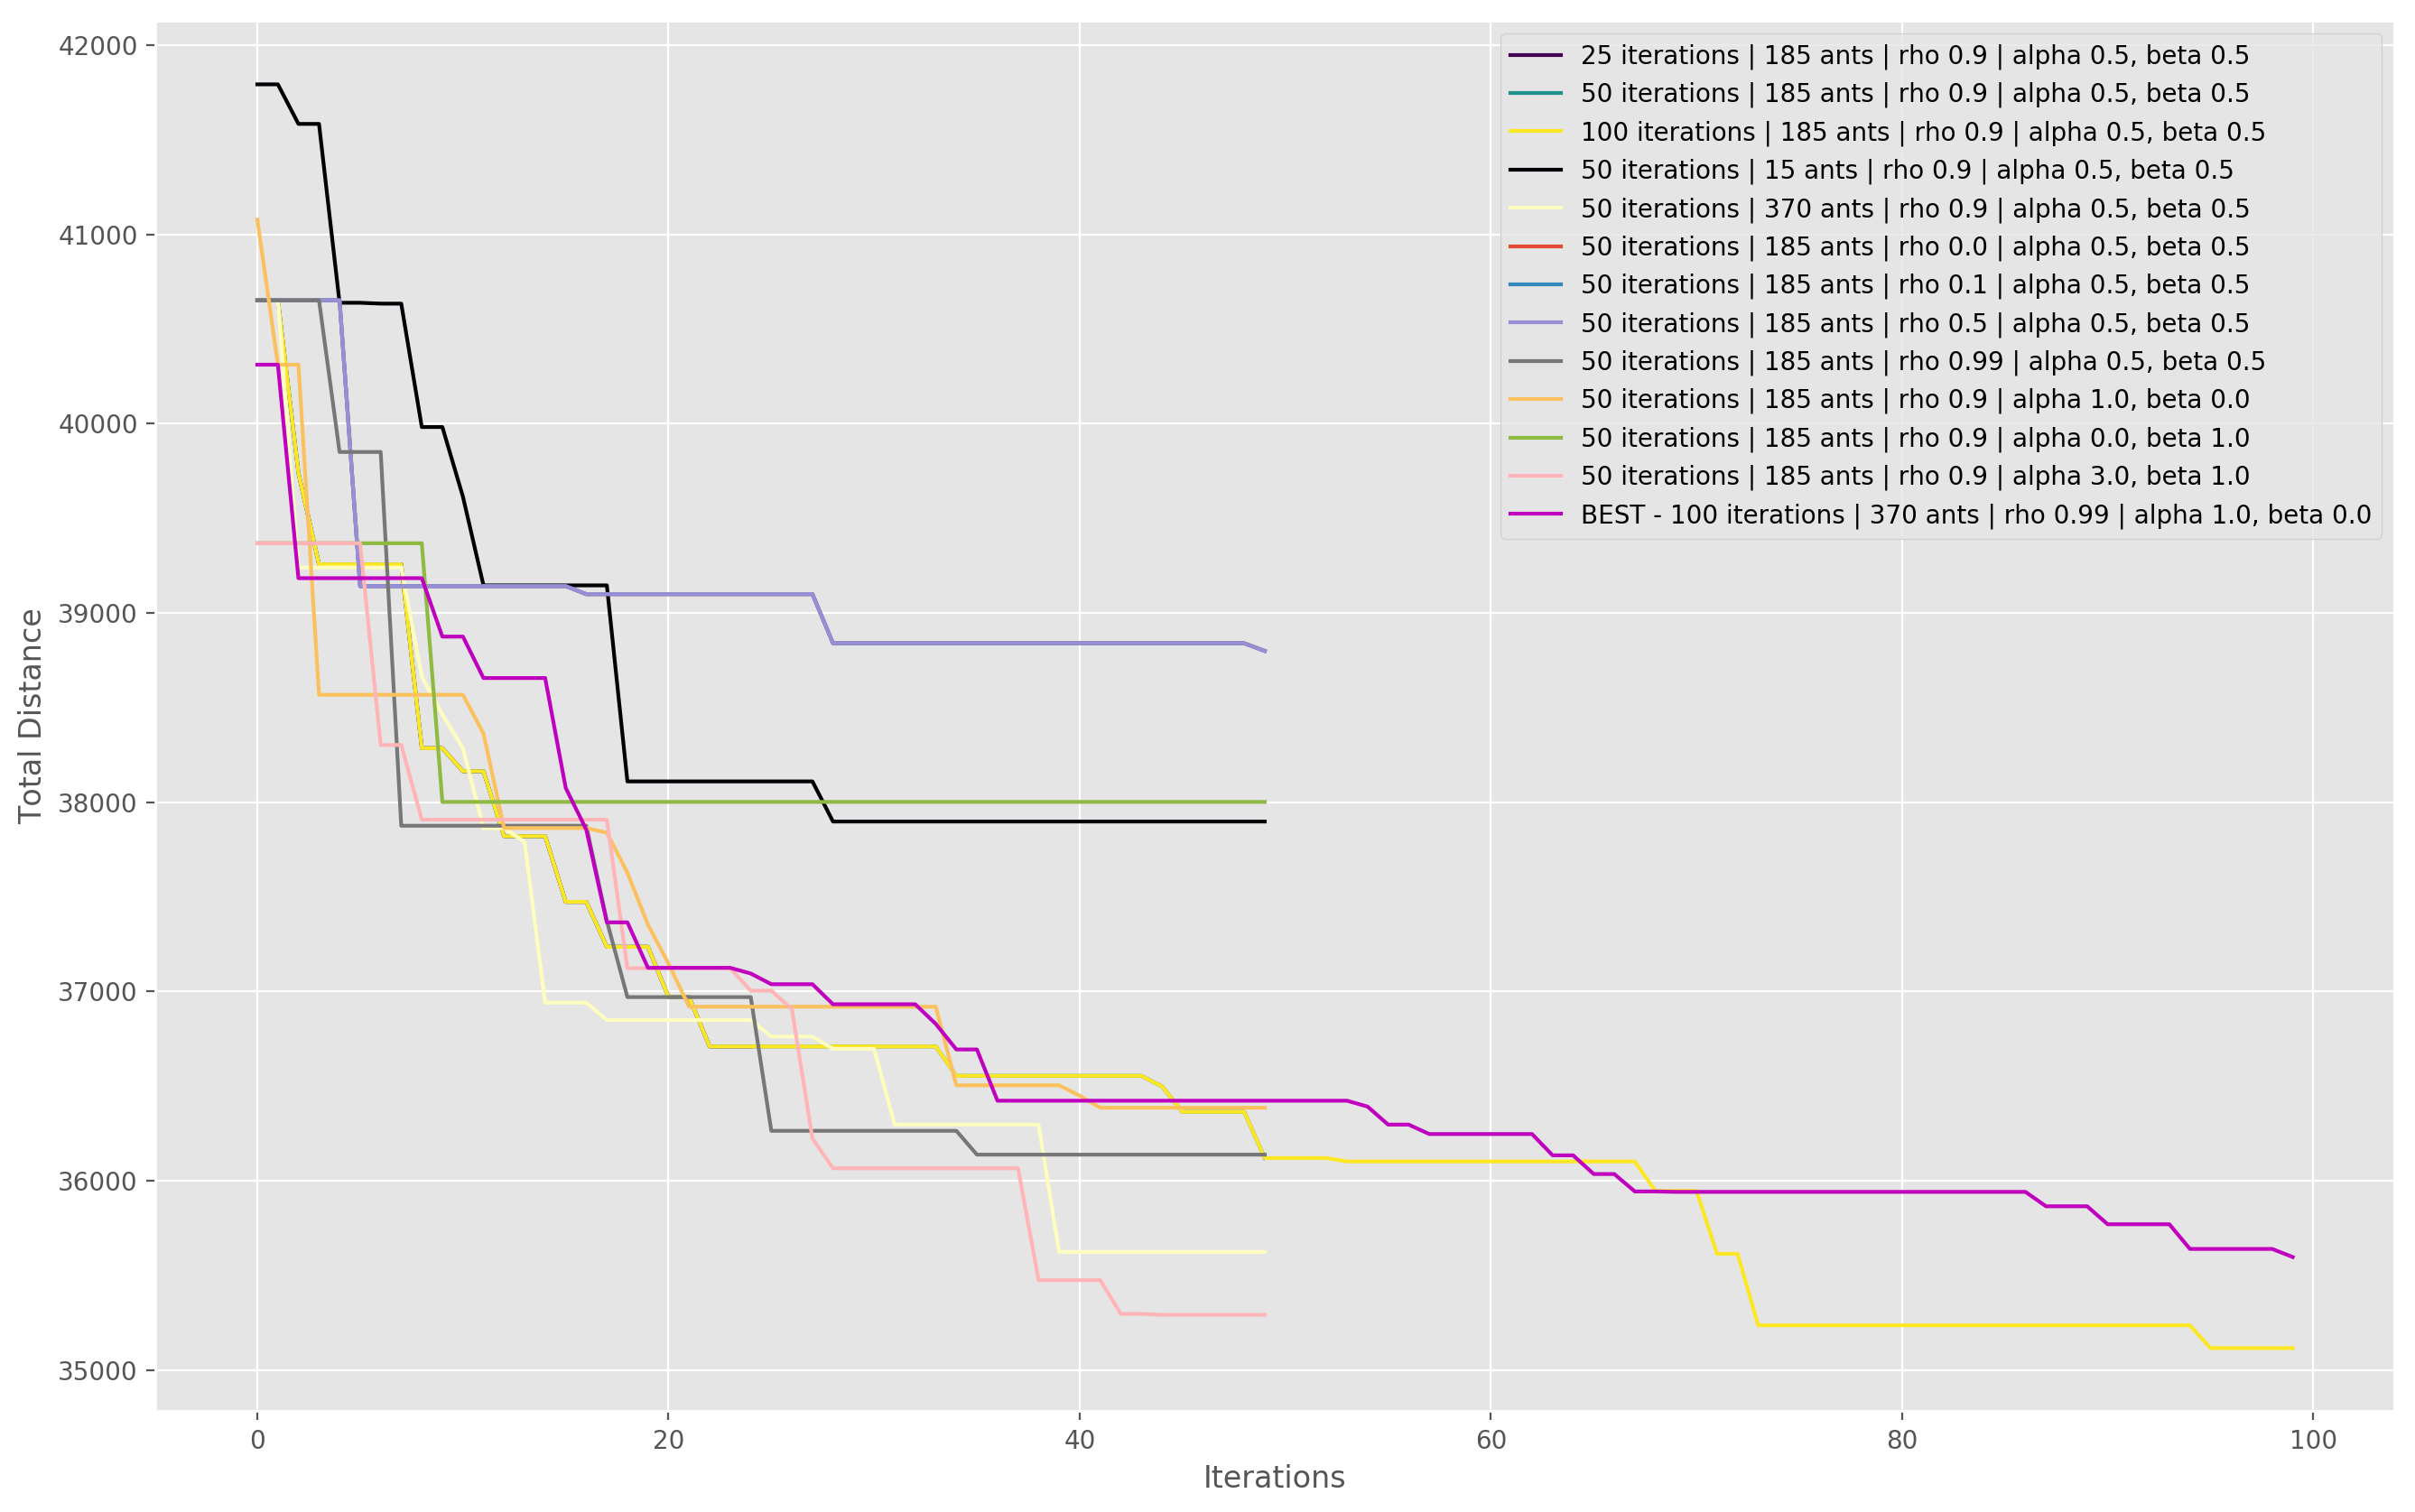
\includegraphics[width=11cm,keepaspectratio]{images/SJC2_best.png}
  \caption{Melhores soluções encontradas para a base SJC2 ao longo das repetições para todas as variações de parâmetros apresentadas até agora.}
  \label{fig:sjc2_best}
\end{figure}

\subsubsection{SJC3b}
A base de dados SJC3b é composta de 300 pontos, todos com capacidade 740, mas com demanda variável. Ela busca por 30 pontos de mediana. A análise da otimização das funções com relação ao número de iterações pode ser vista na Figura \ref{fig:sjc3b_iterations}. Assim como acontece com a base SJC1 quando usados os valores padrões para os parâmetros e 10 formigas, após a iteração 65, e até a iteração final, tanto a média quanto o desvio padrão sofrem um mudança brusca. Isso aconteceu pois em uma das execuções, após essa iteração, a distância total cai de 45726 para 2190. 

\begin{figure}[h]	
  \centering
  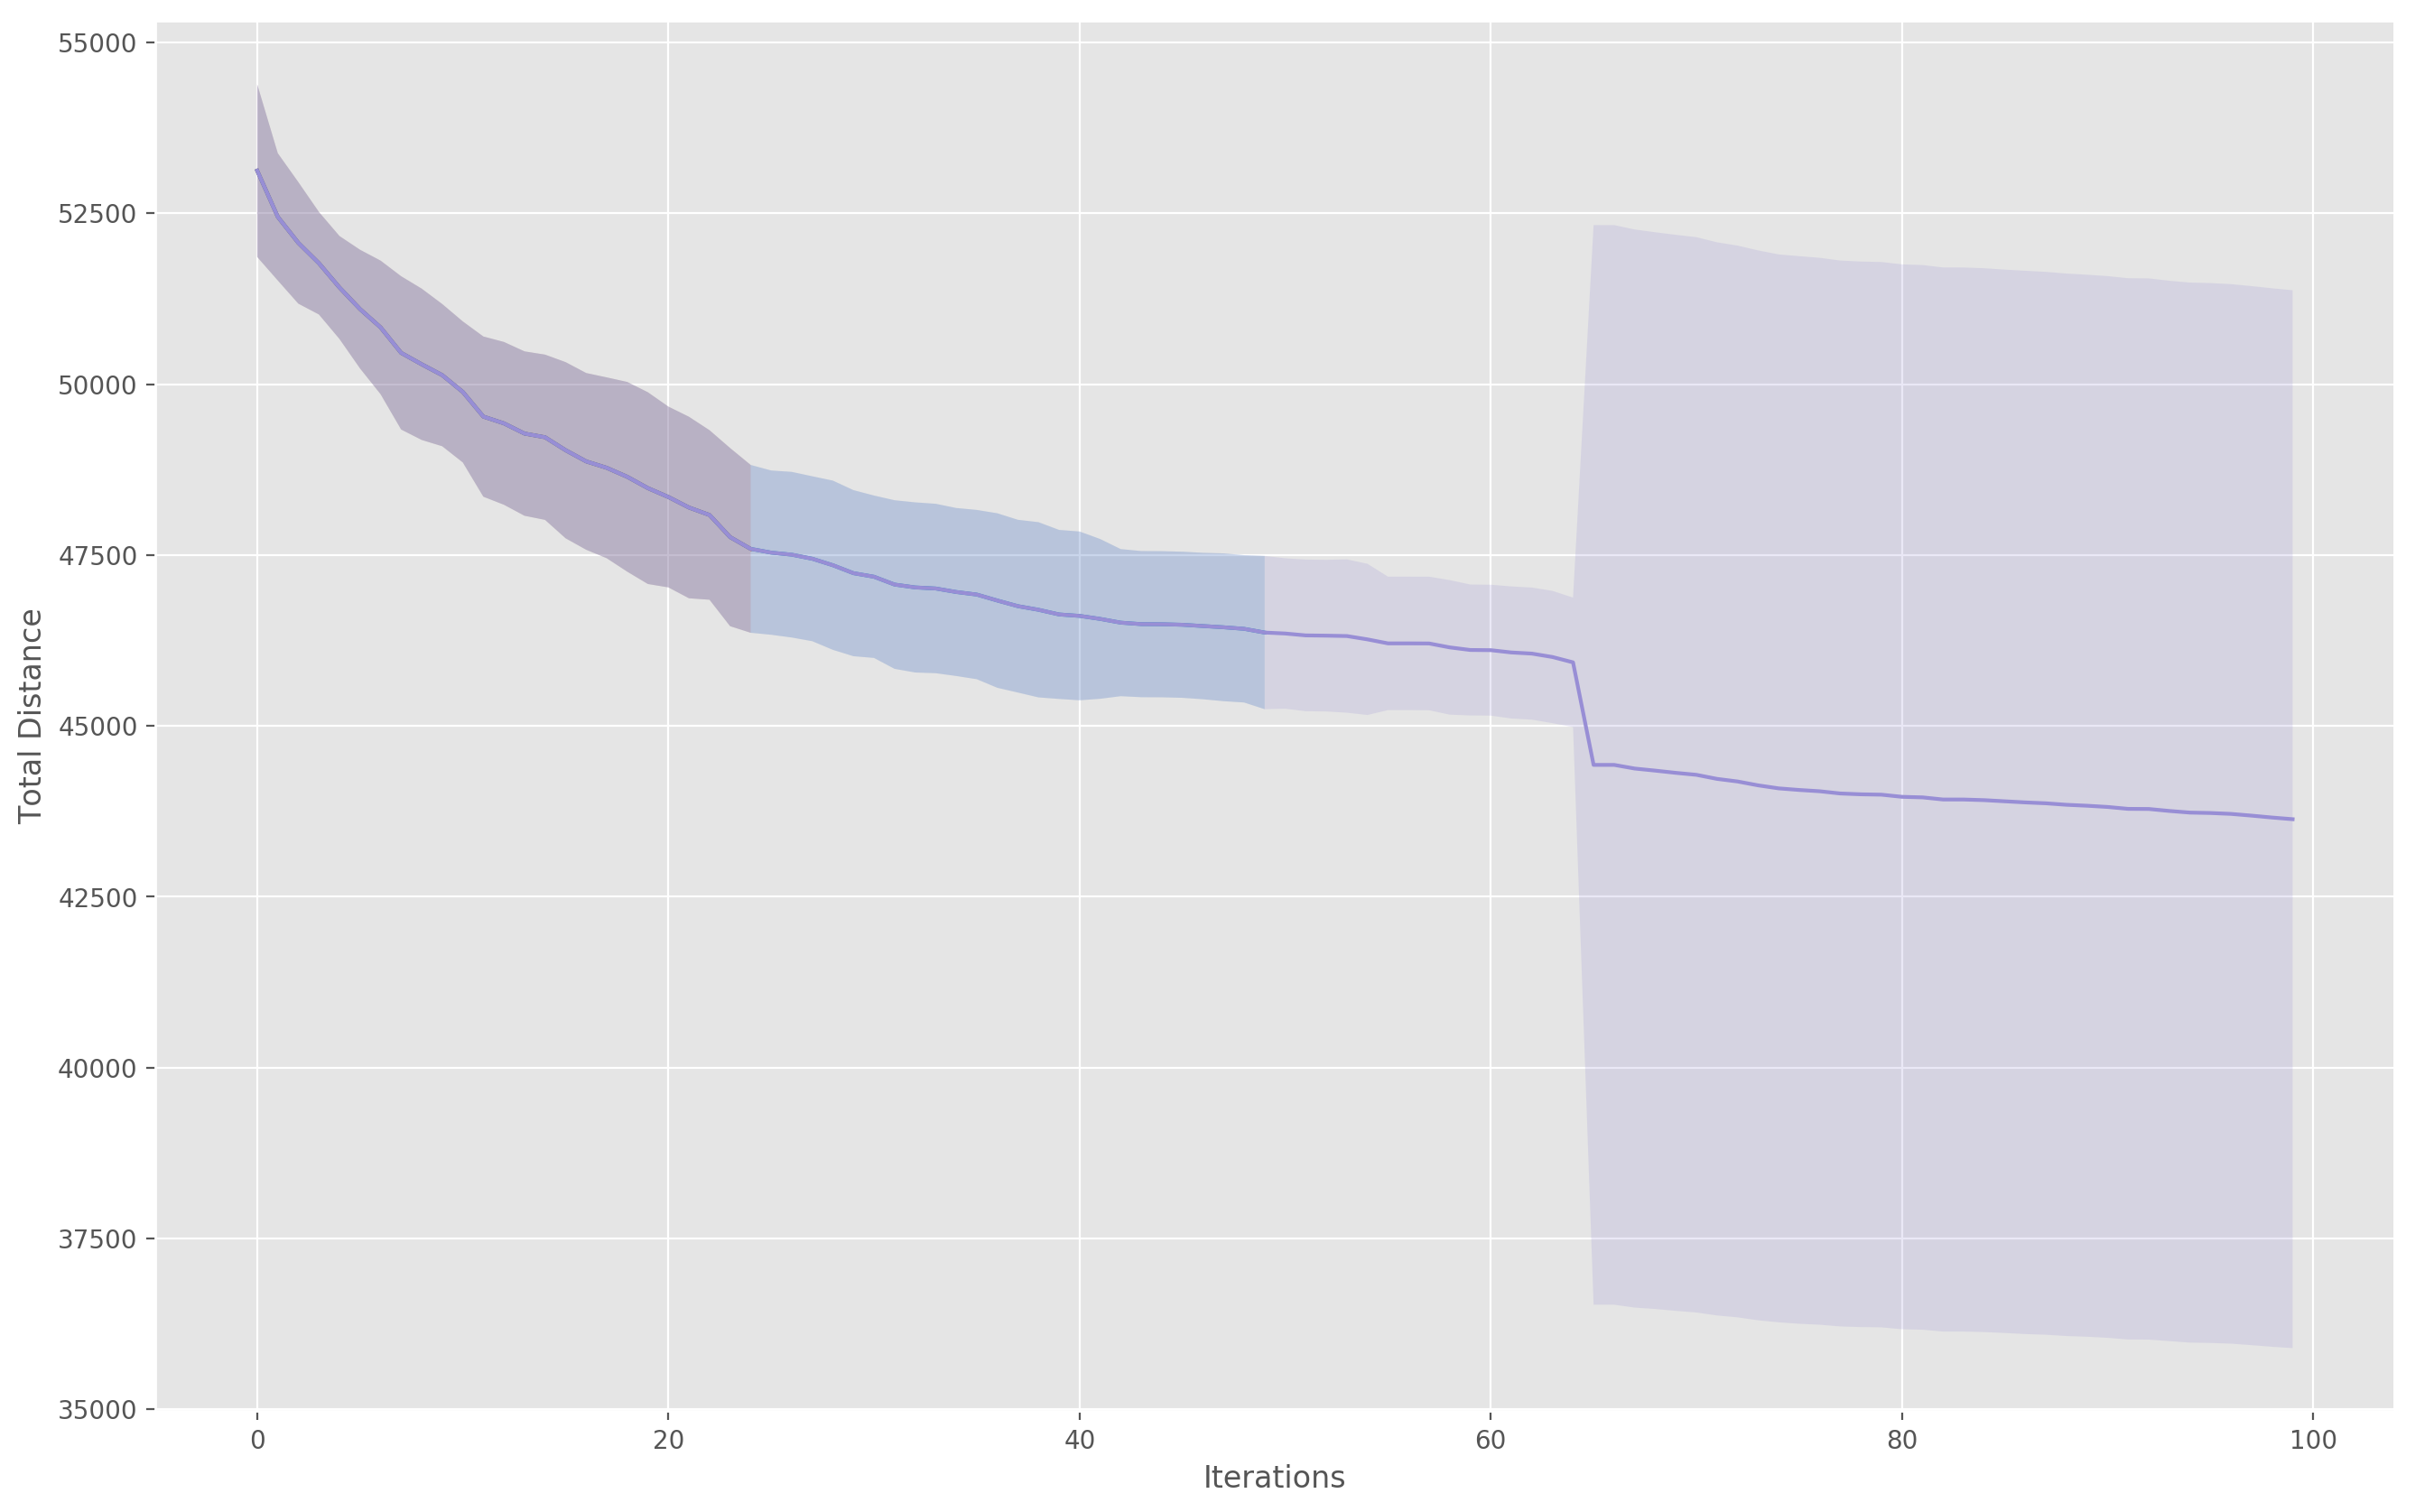
\includegraphics[width=11cm,keepaspectratio]{images/SJC3b_iterations.png}
  \caption{Média e desvio padrão para a distância da solução encontrada para base SJC3b com número de iterações variável.}
  \label{fig:sjc3b_iterations}
\end{figure}

Neste momento o leitor pode se perguntar o porque não apresentamos resultados para um número de iterações acima de 100. Não o fizemos pois, com um número 5 vezes maior de iterações, acaba que ocorre erro em todas as repetições, portanto a média do melhor global termina em 2190, como podemos ver na Figura \ref{fig:sjc3b_fail}. Esses gráficos não nos ajudam na análise, e portanto foram descartados.

\begin{figure}[h]	
  \centering
  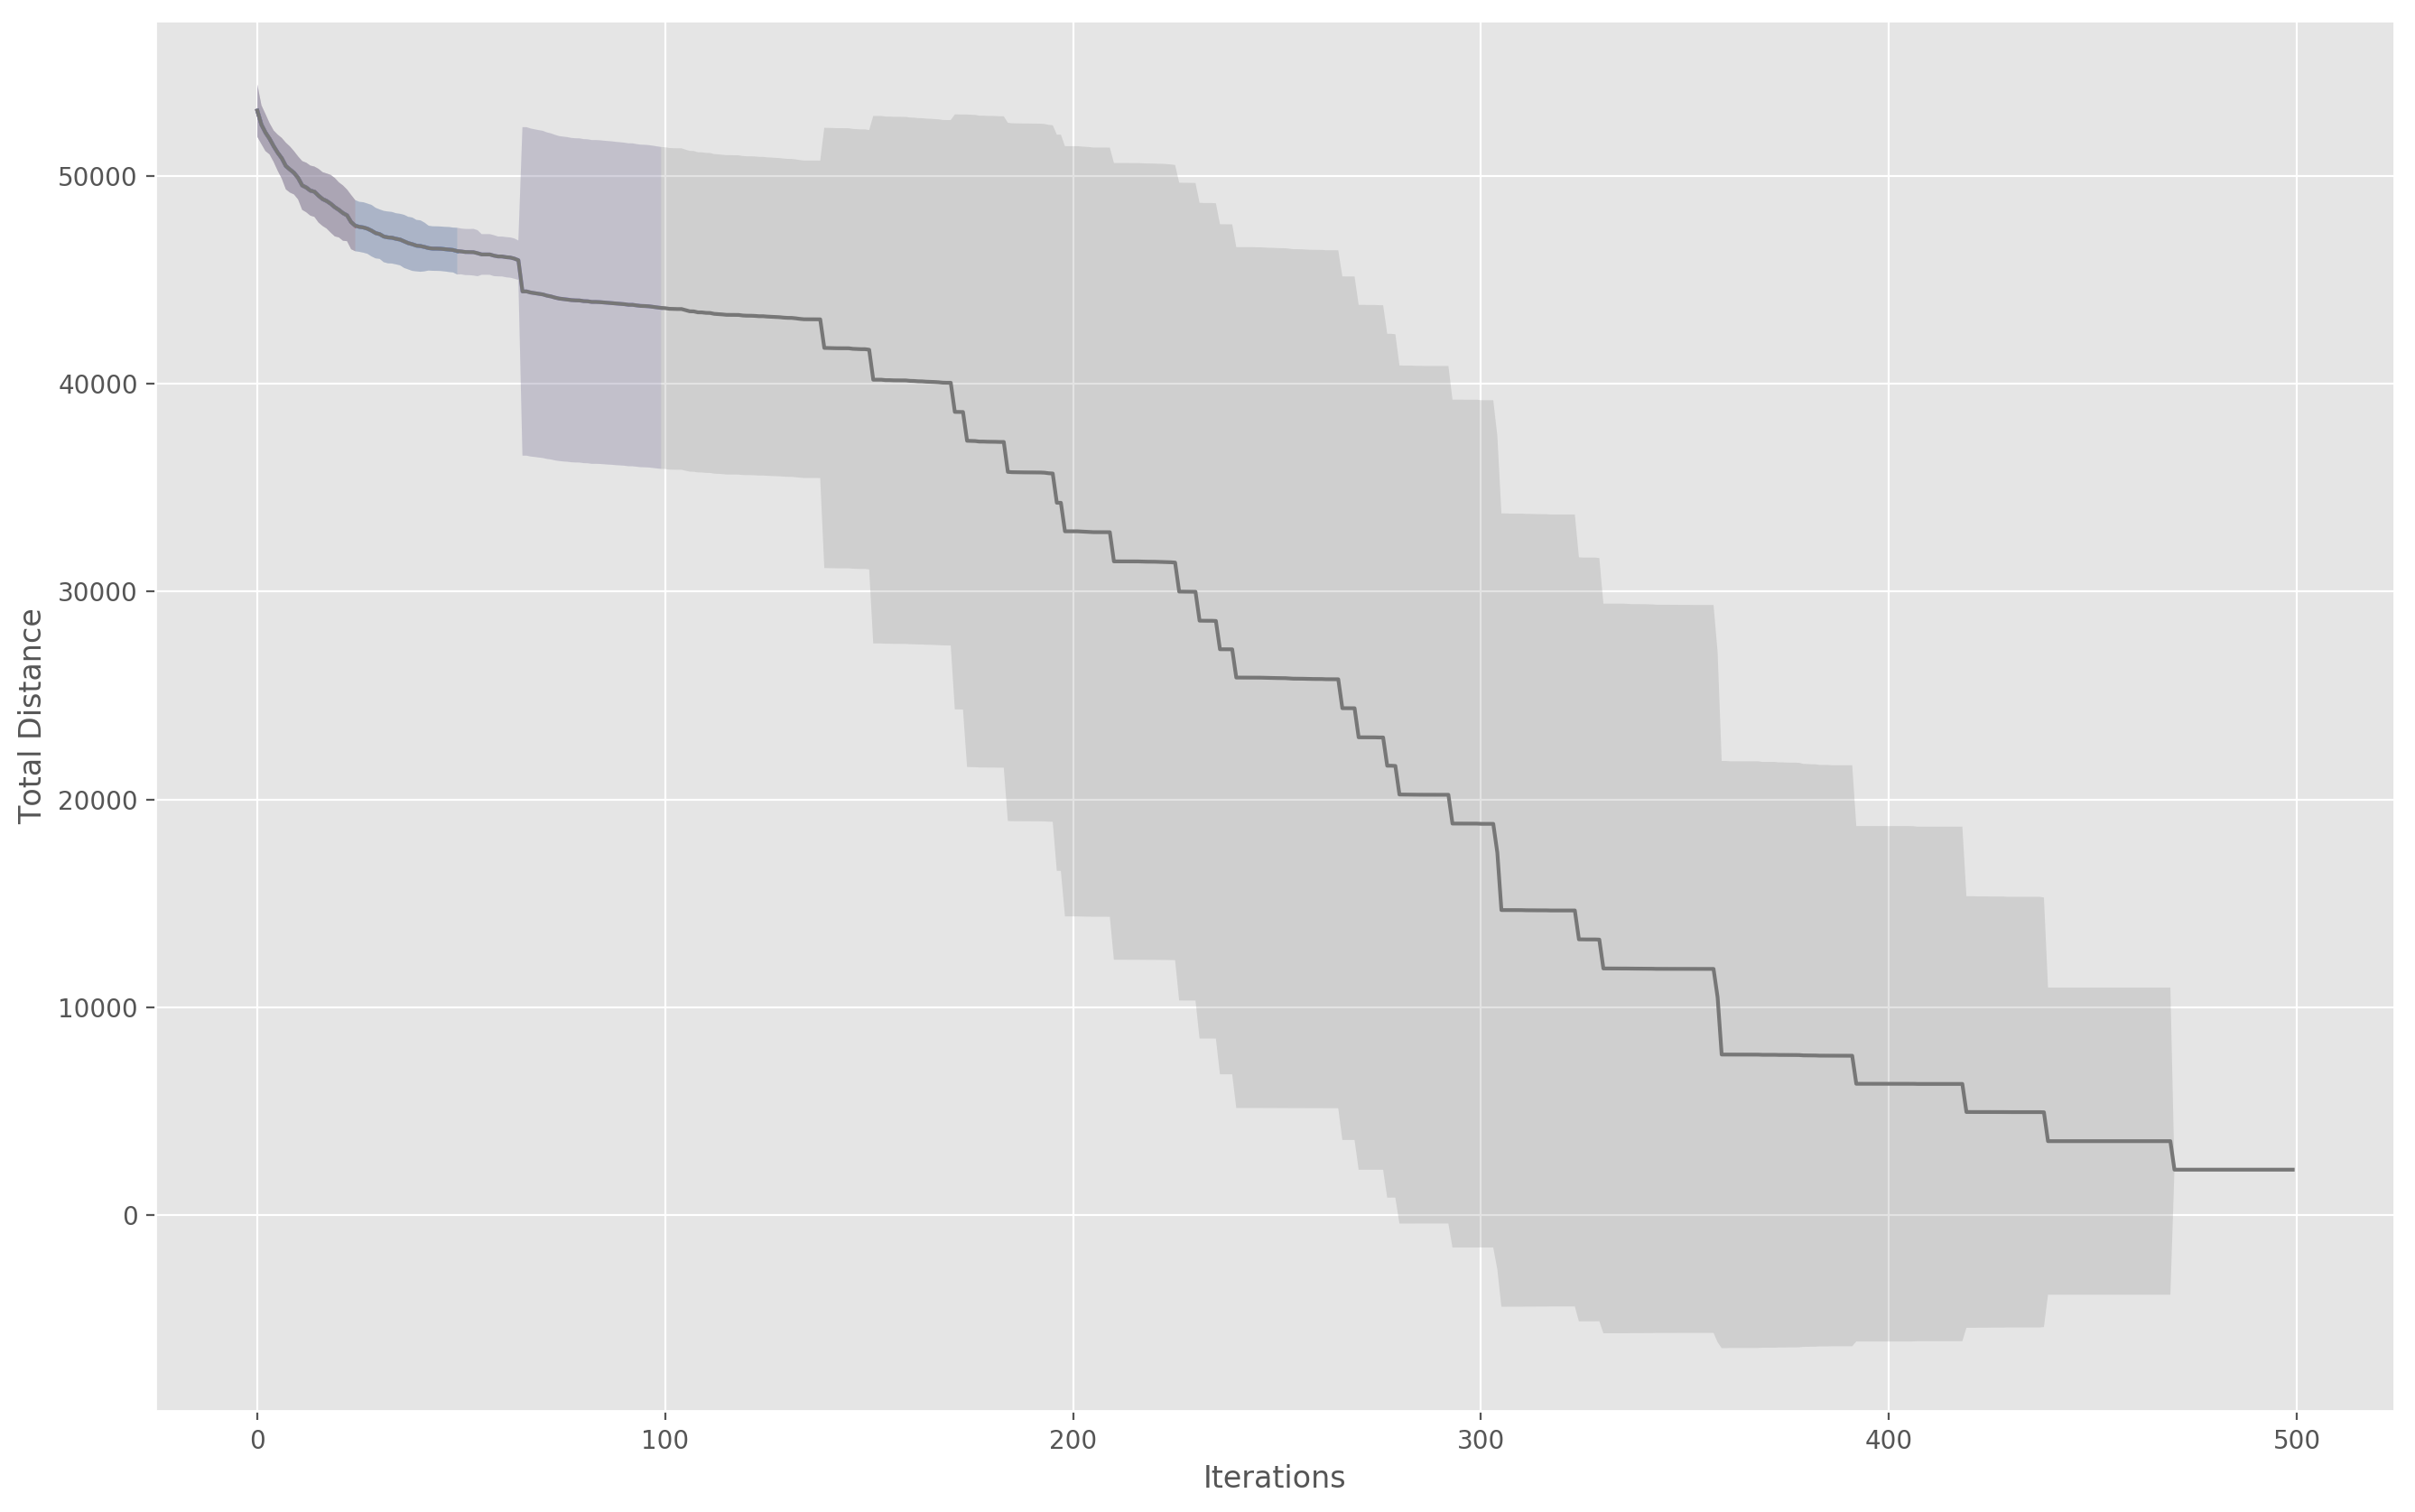
\includegraphics[width=11cm,keepaspectratio]{images/SJC3b_iterations_fail.png}
  \caption{Média e desvio padrão para a distância da solução encontrada para base SJC3b com número de formigas variável.}
  \label{fig:sjc3b_fail}
\end{figure}

No gráfico da Figura \ref{fig:sjc3b_ants} vemos que o erro ocorre novamente. No entanto, mesmo antes disso o valor médio da melhor solução global já era superior a todos os outros, fazendo com que, mais uma vez $2 * (n - p)$ formigas seja o ideal.

\begin{figure}[h]	
  \centering
  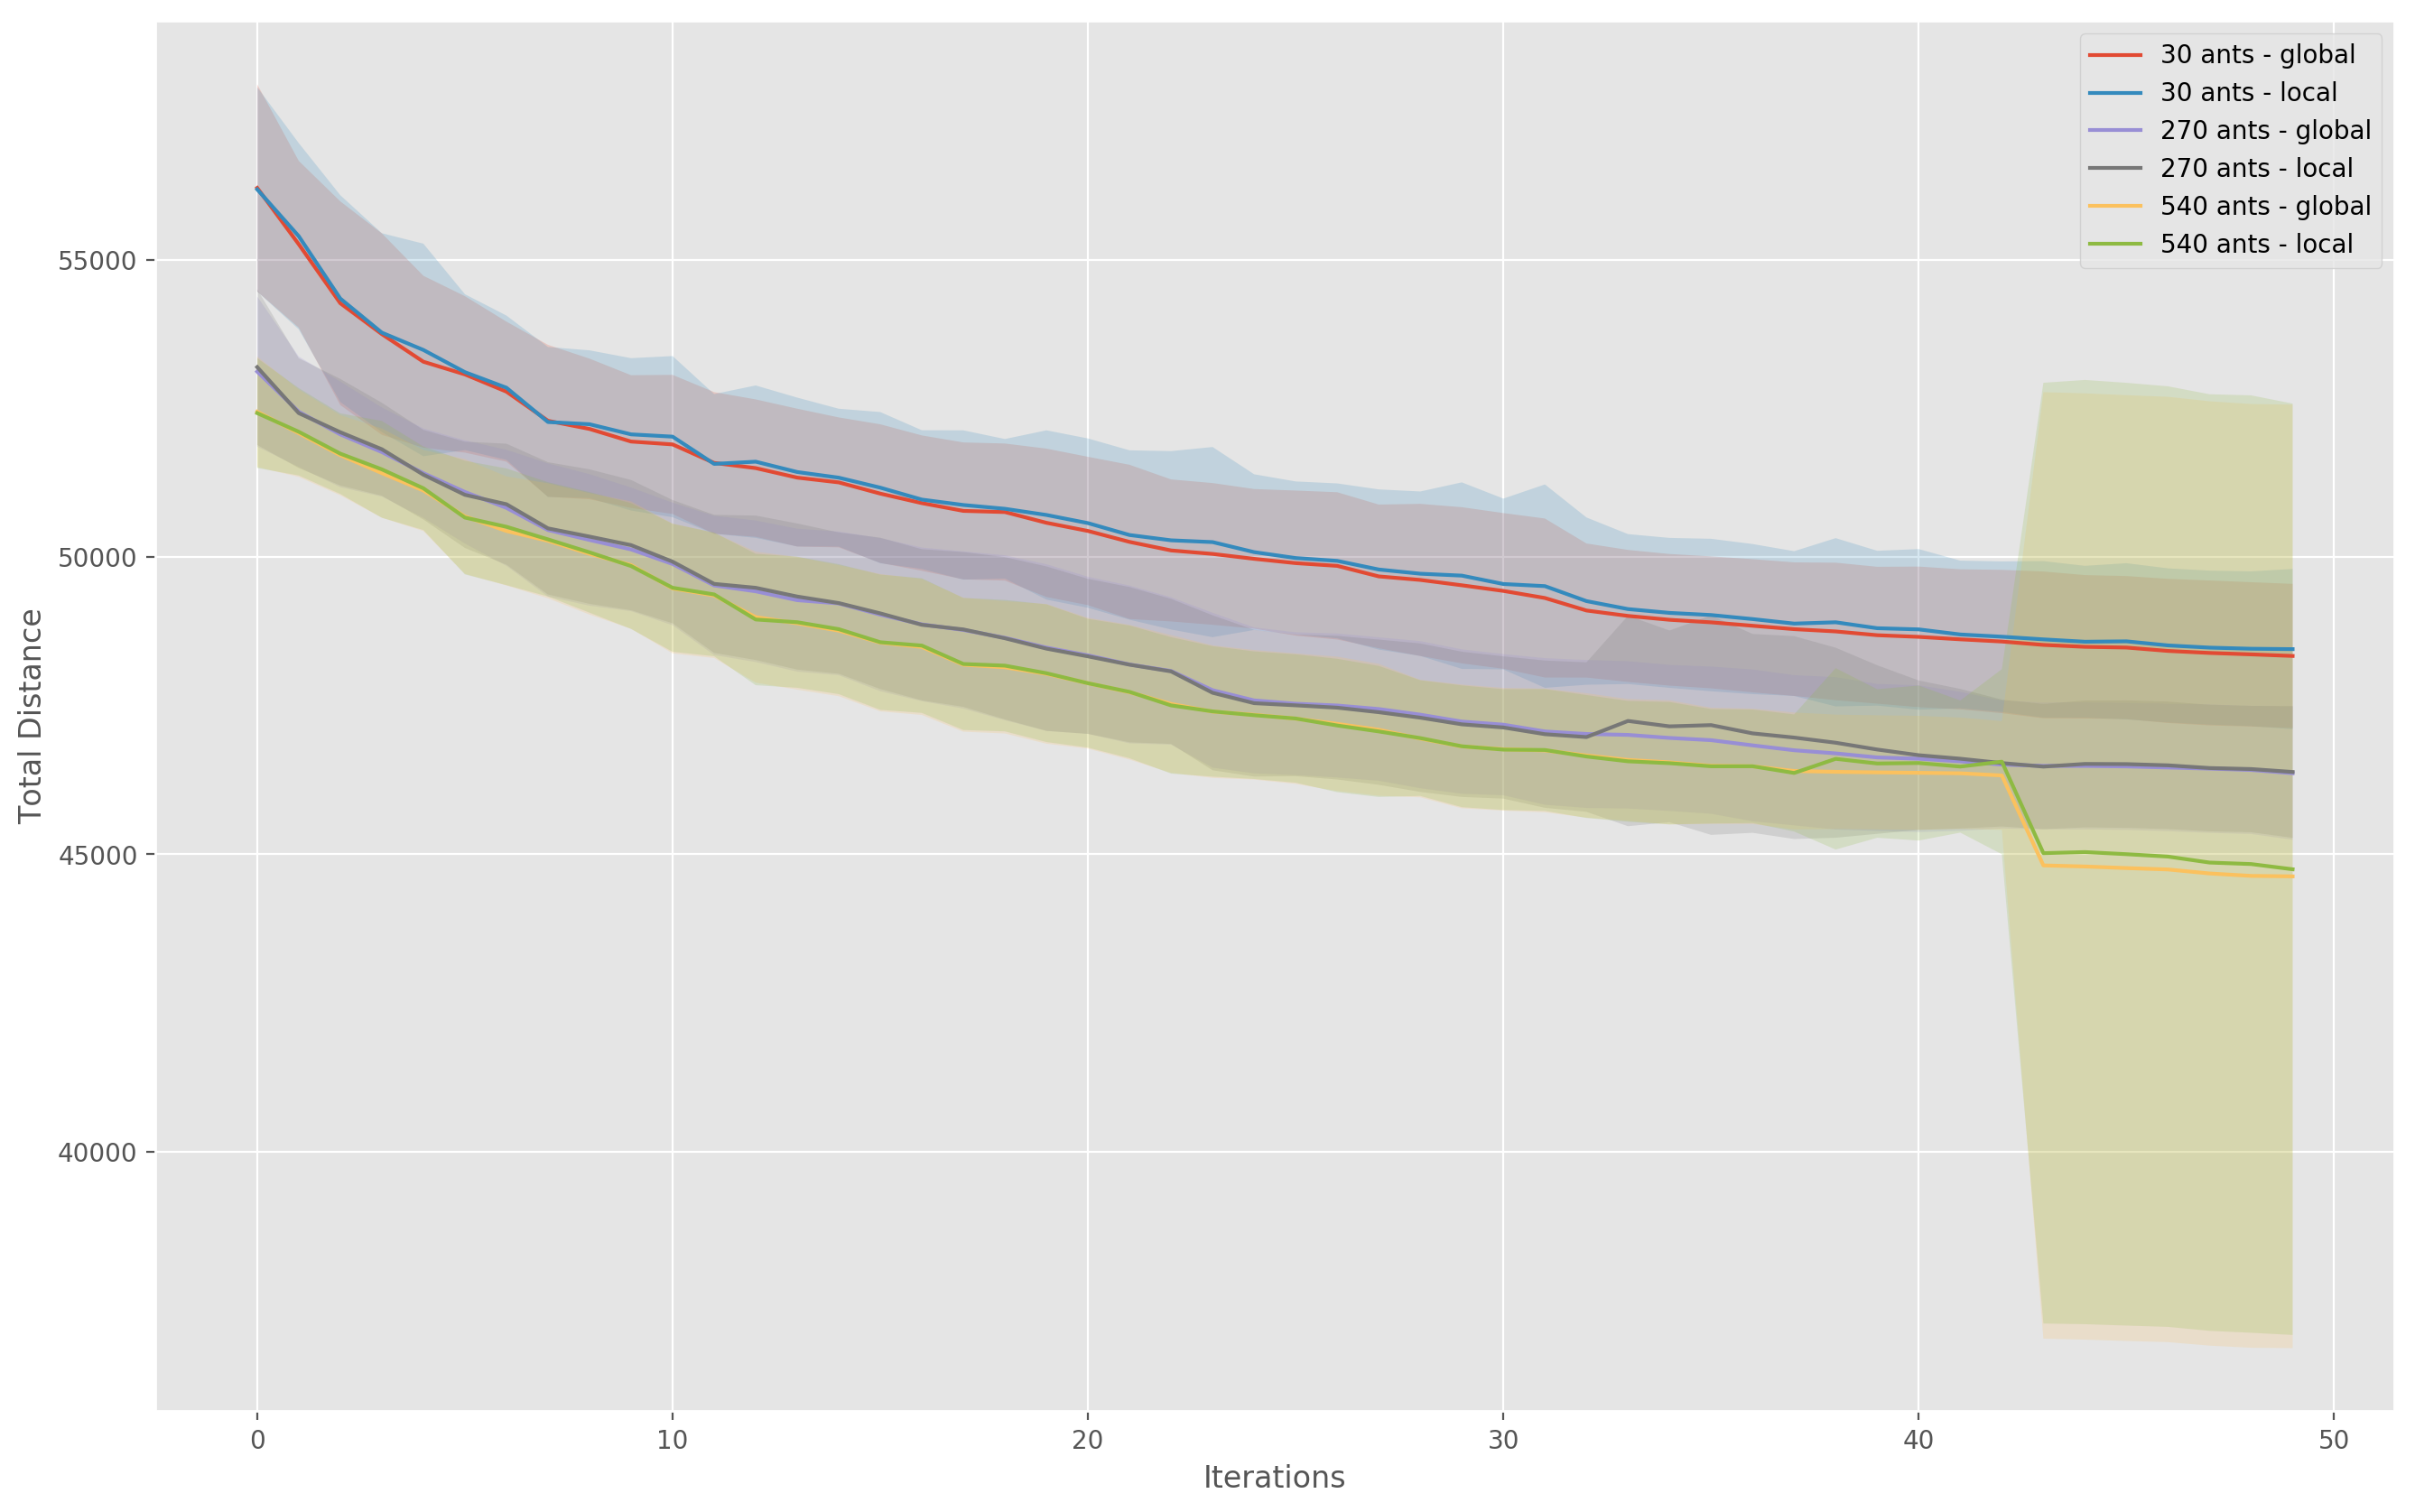
\includegraphics[width=11cm,keepaspectratio]{images/SJC3b_ants.png}
  \caption{Média e desvio padrão para a distância da solução encontrada para base SJC3b com número de formigas variável.}
  \label{fig:sjc3b_ants}
\end{figure}

Para variação da taxa de evaporação temos um cenário(Figura \ref{fig:sjc3b_rho}) semelhante às outras duas bases, porém dessa vez $\rho = 0.9$ se sobressaiu dos demais.

\begin{figure}[h]	
  \centering
  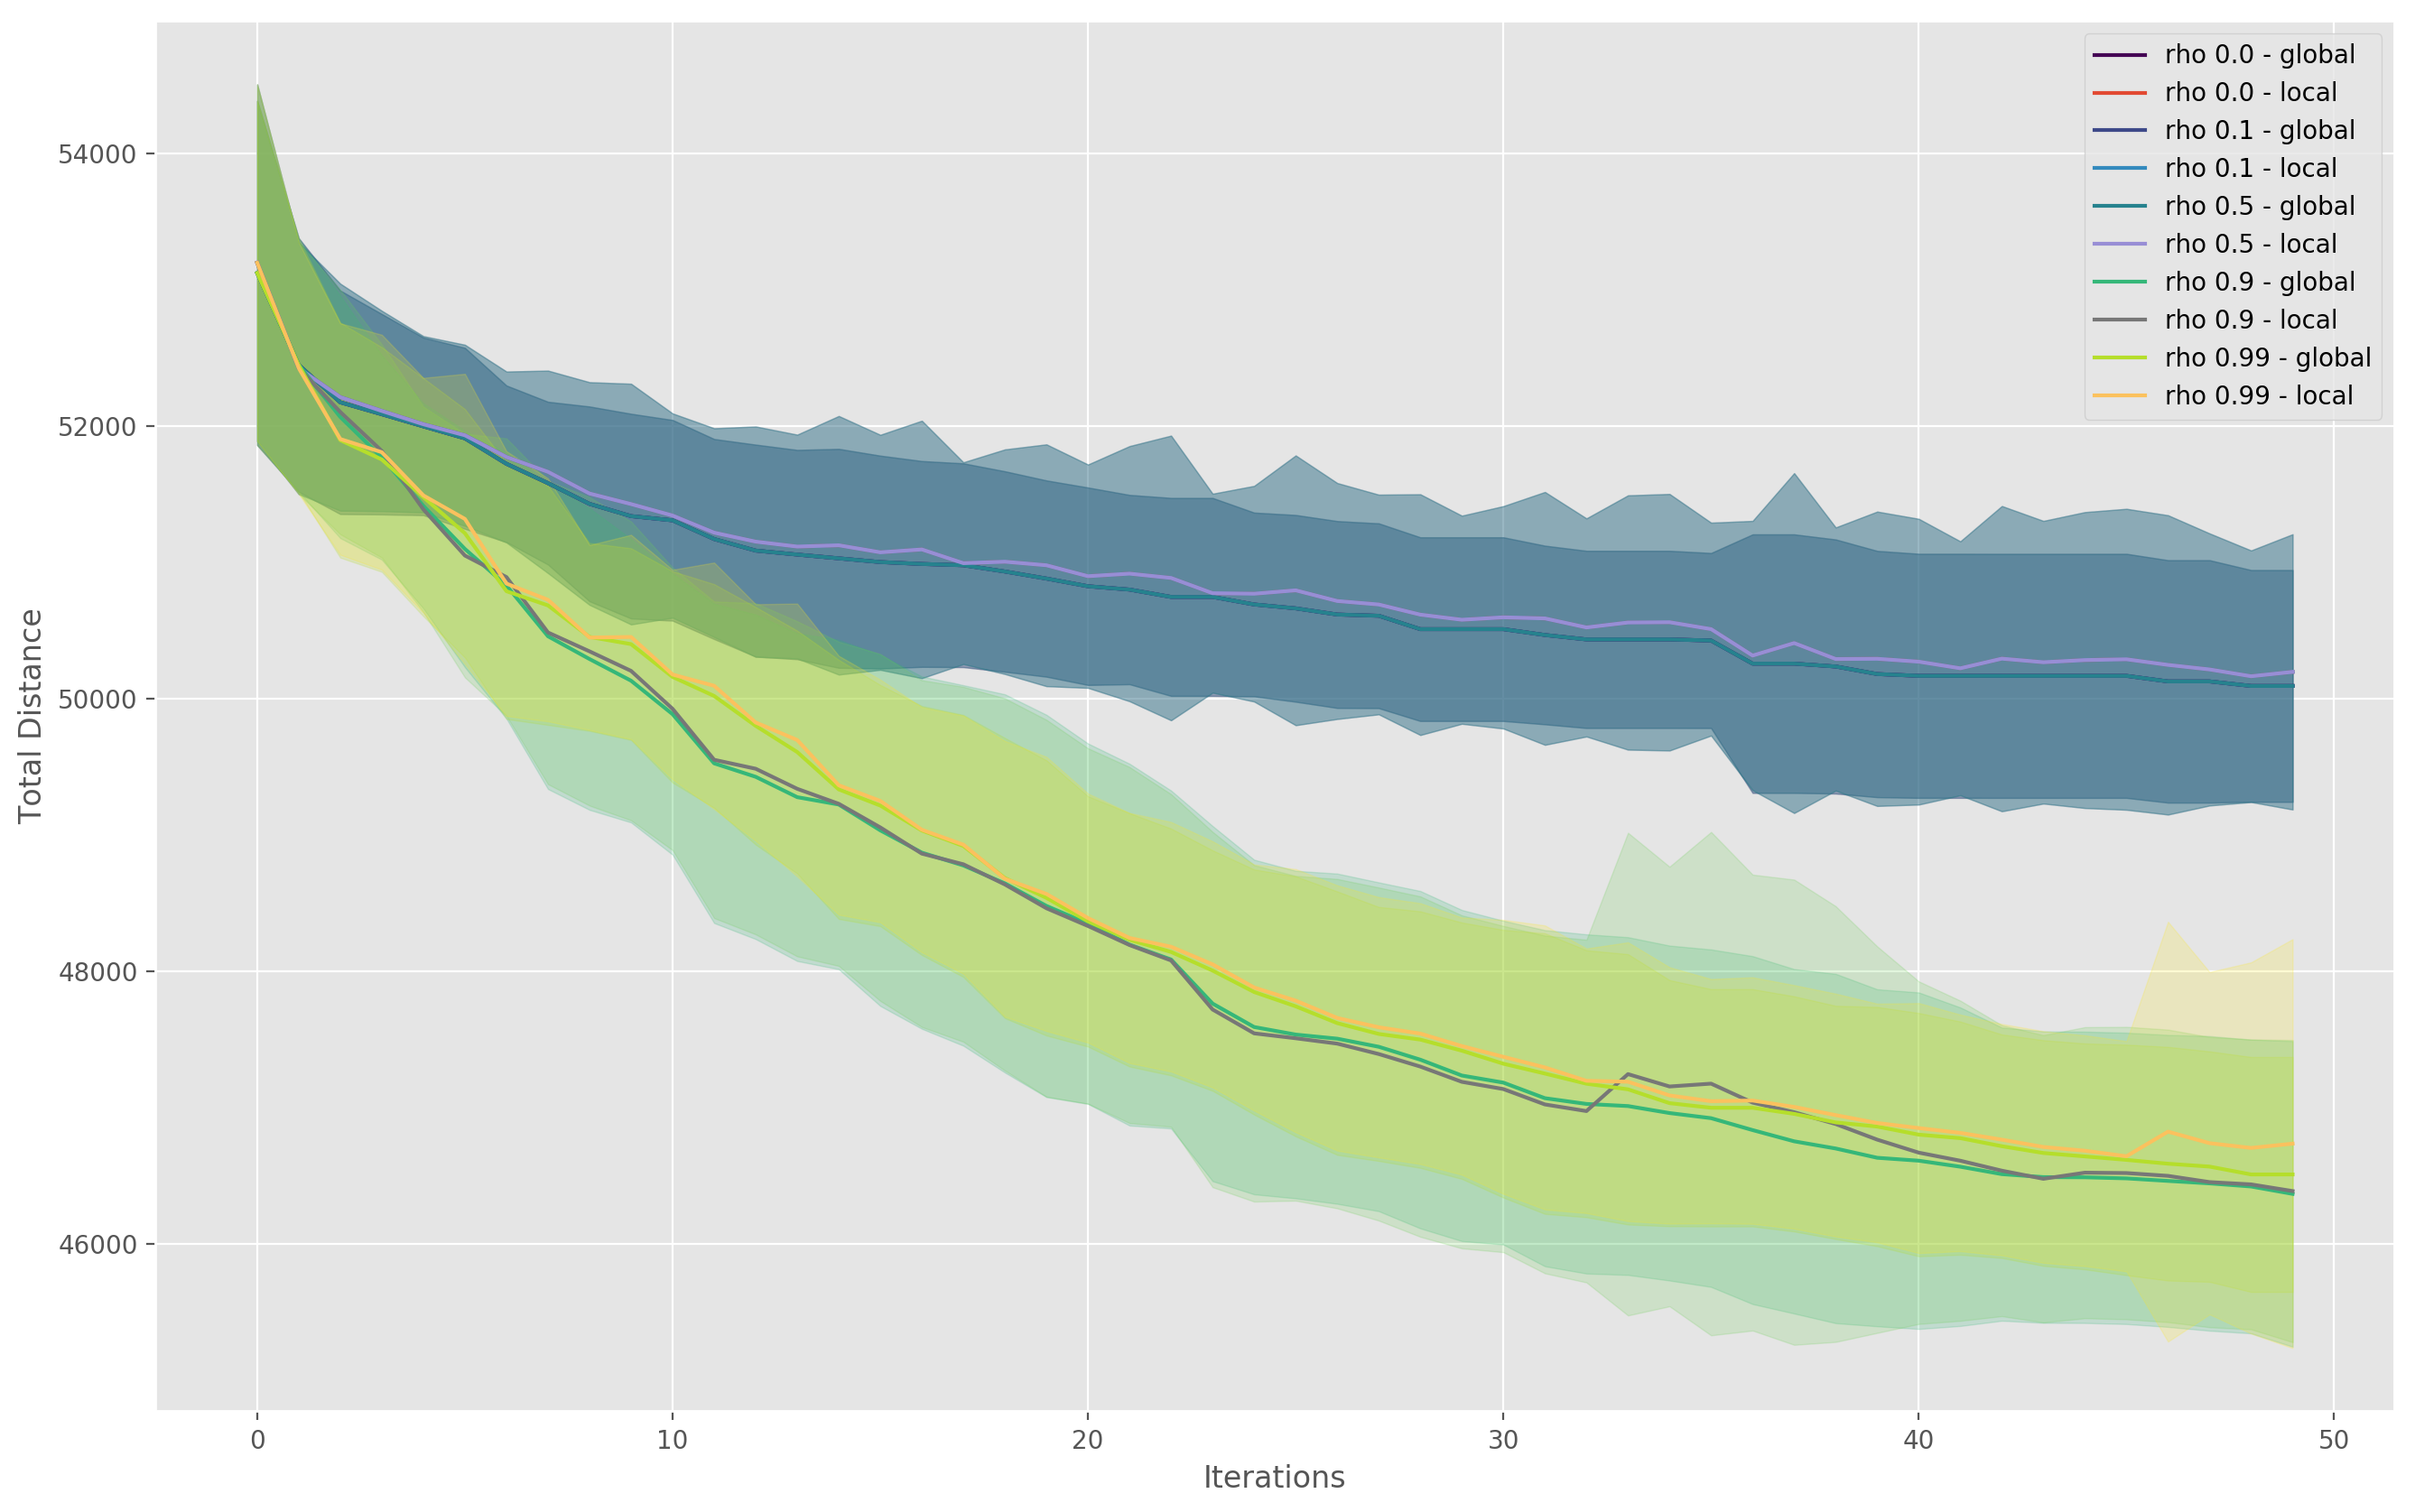
\includegraphics[width=11cm,keepaspectratio]{images/SJC3b_rho.png}
  \caption{Média e desvio padrão para a distância da solução encontrada para base SJC3b com taxa de evaporação de feromônio variável.}
  \label{fig:sjc3b_rho}
\end{figure}

Na análise dos termos $\alpha$ e $\beta$, é fácil perceber pela Figura \ref{fig:sjc3b_alpha_beta} que os parâmetros ótimos são $\alpha = 3$ e $\beta = 1$, reforçando os achados de \cite{de2005max}.

\begin{figure}[h]	
  \centering
  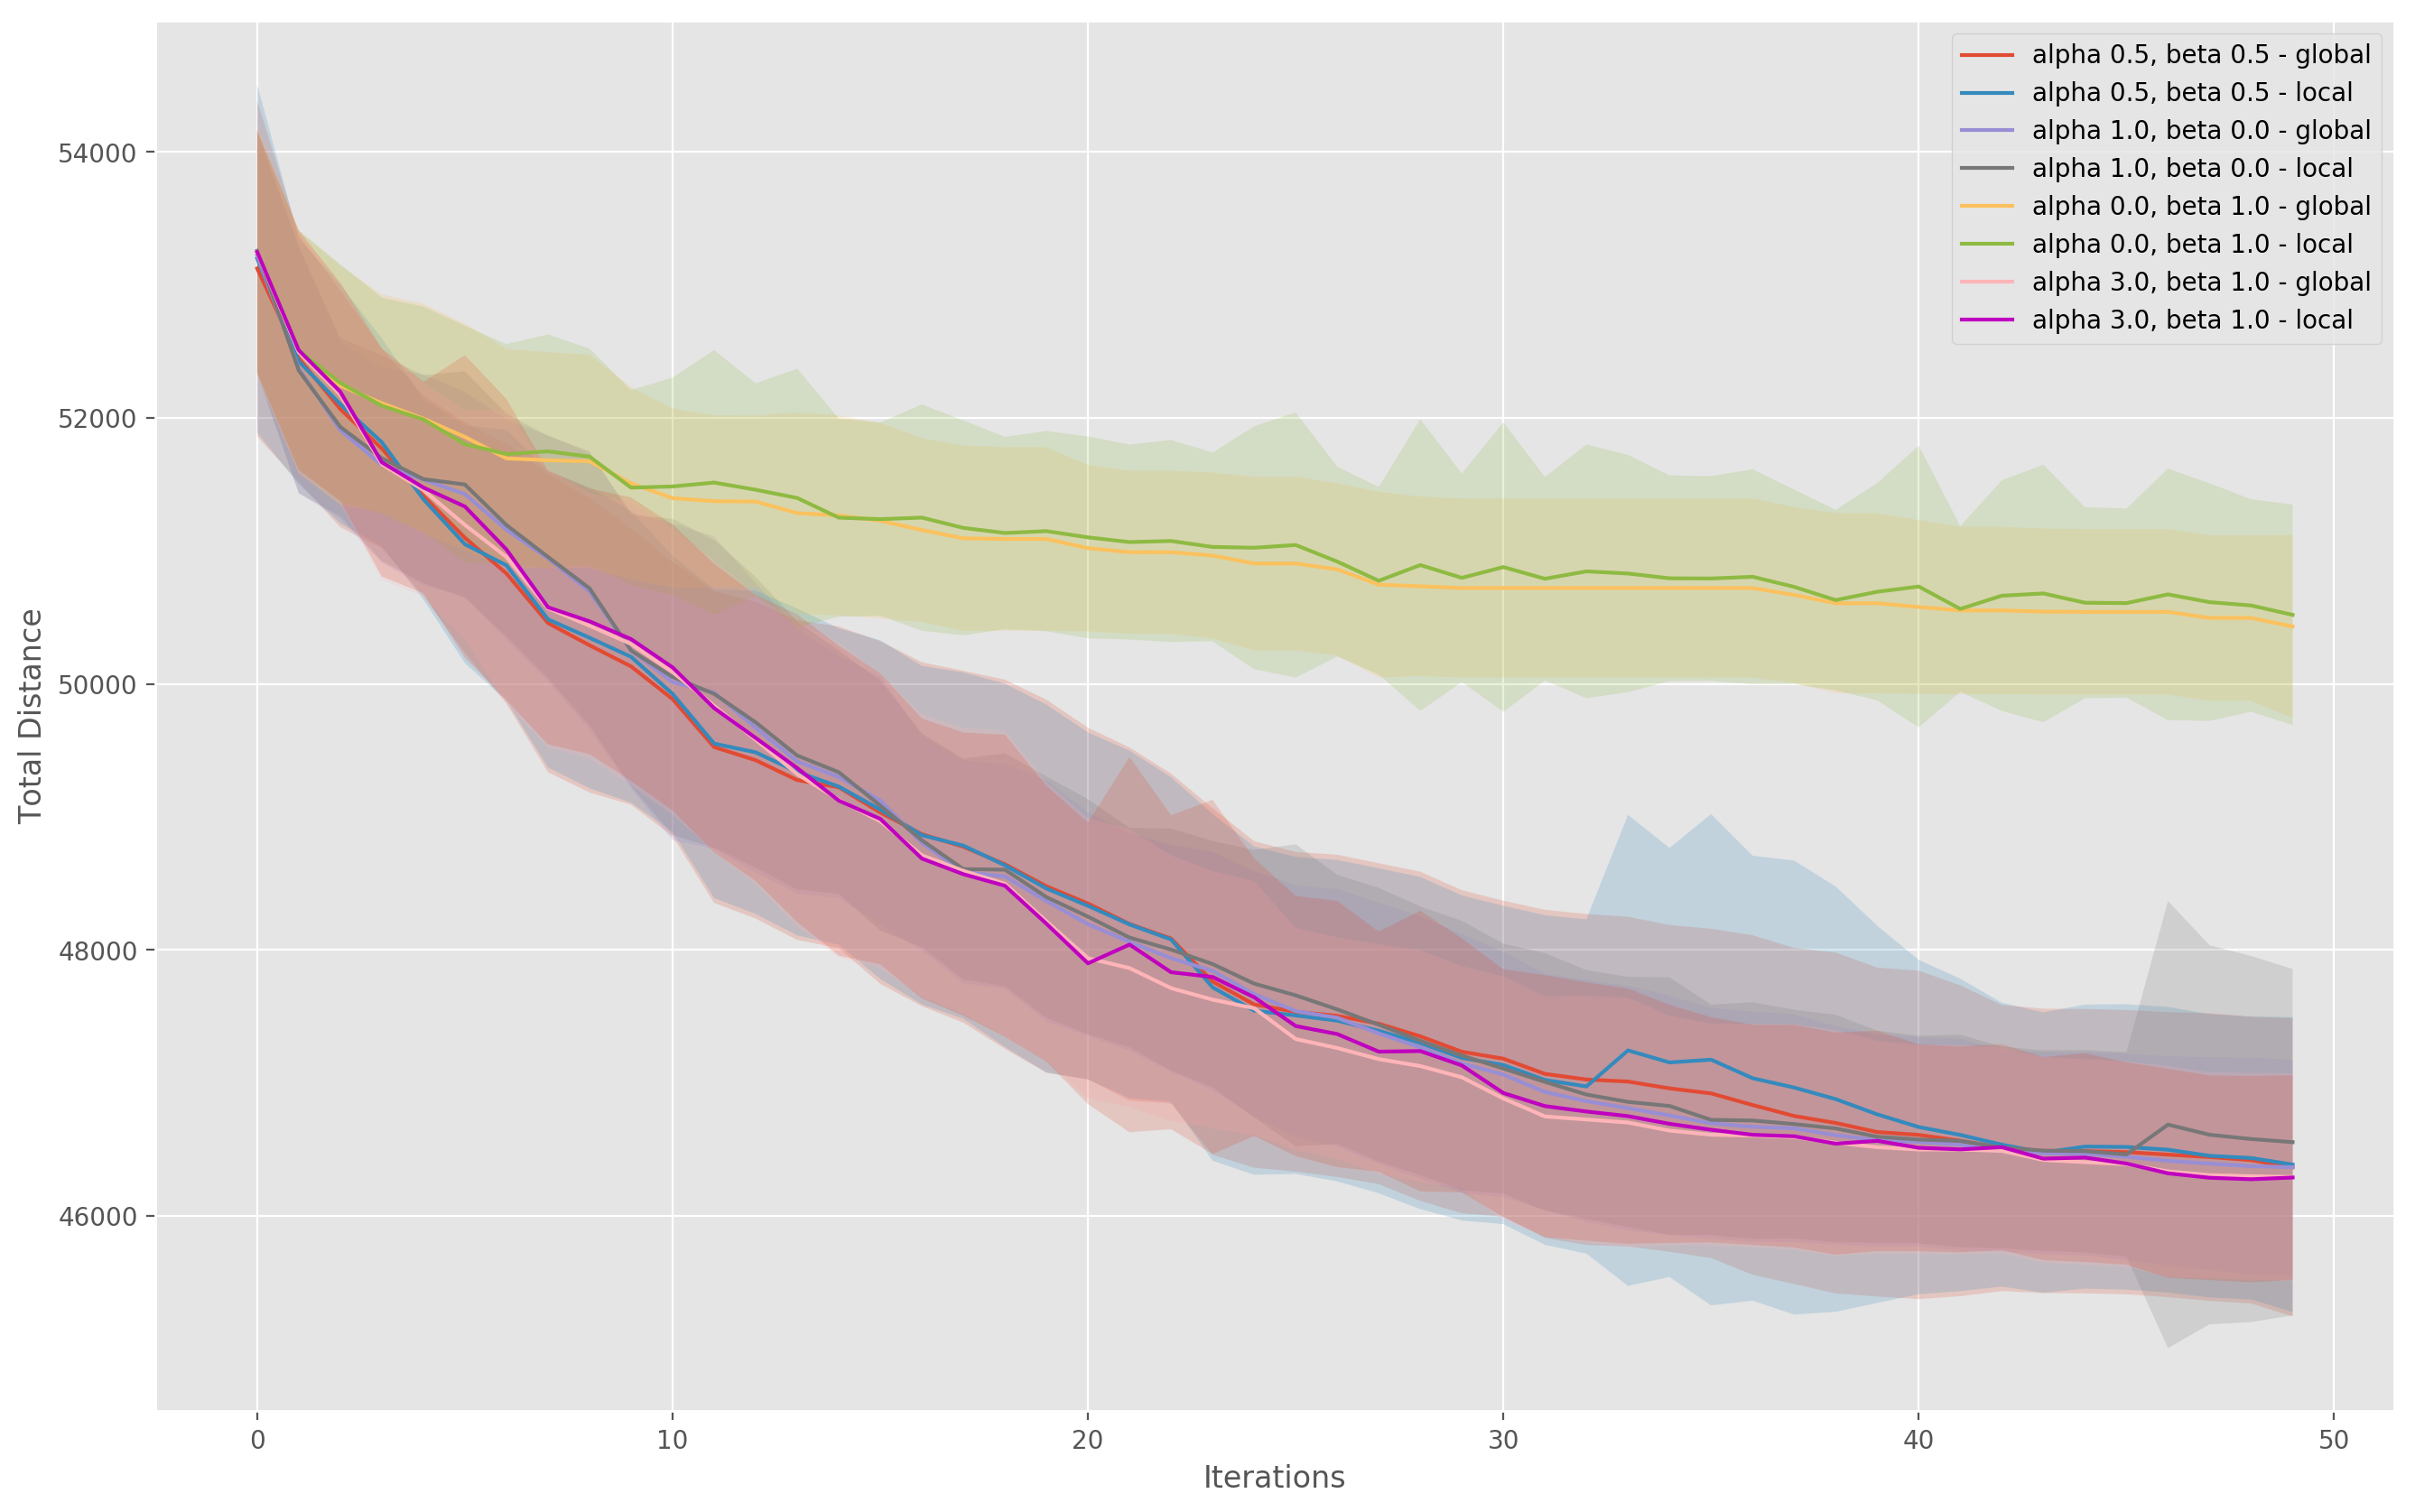
\includegraphics[width=11cm,keepaspectratio]{images/SJC3b_alpha_beta.png}
  \caption{Média e desvio padrão para a distância da solução encontrada para base SJC3b com a variação dos pesos dos feromônios e da heurística de informação no cálculo da probabilidade de escolha do nó.}
  \label{fig:sjc3b_alpha_beta}
\end{figure}

Os melhores parâmetros para a base SJC3b foram, portanto, 100 iterações, 540 formigas, $\rho = 0.9$, $\alpha=3$ e $\beta=1$. A Figura \ref{fig:sjc3b_best} mostra os melhores resultados alcançados para cada configuração. Ignorando os dois resultados bugados, vemos que a melhor solução de todas, de valor \textbf{43786.659}, foi encontrada com o conjunto dos melhores parâmetros.

\begin{figure}[h]	
  \centering
  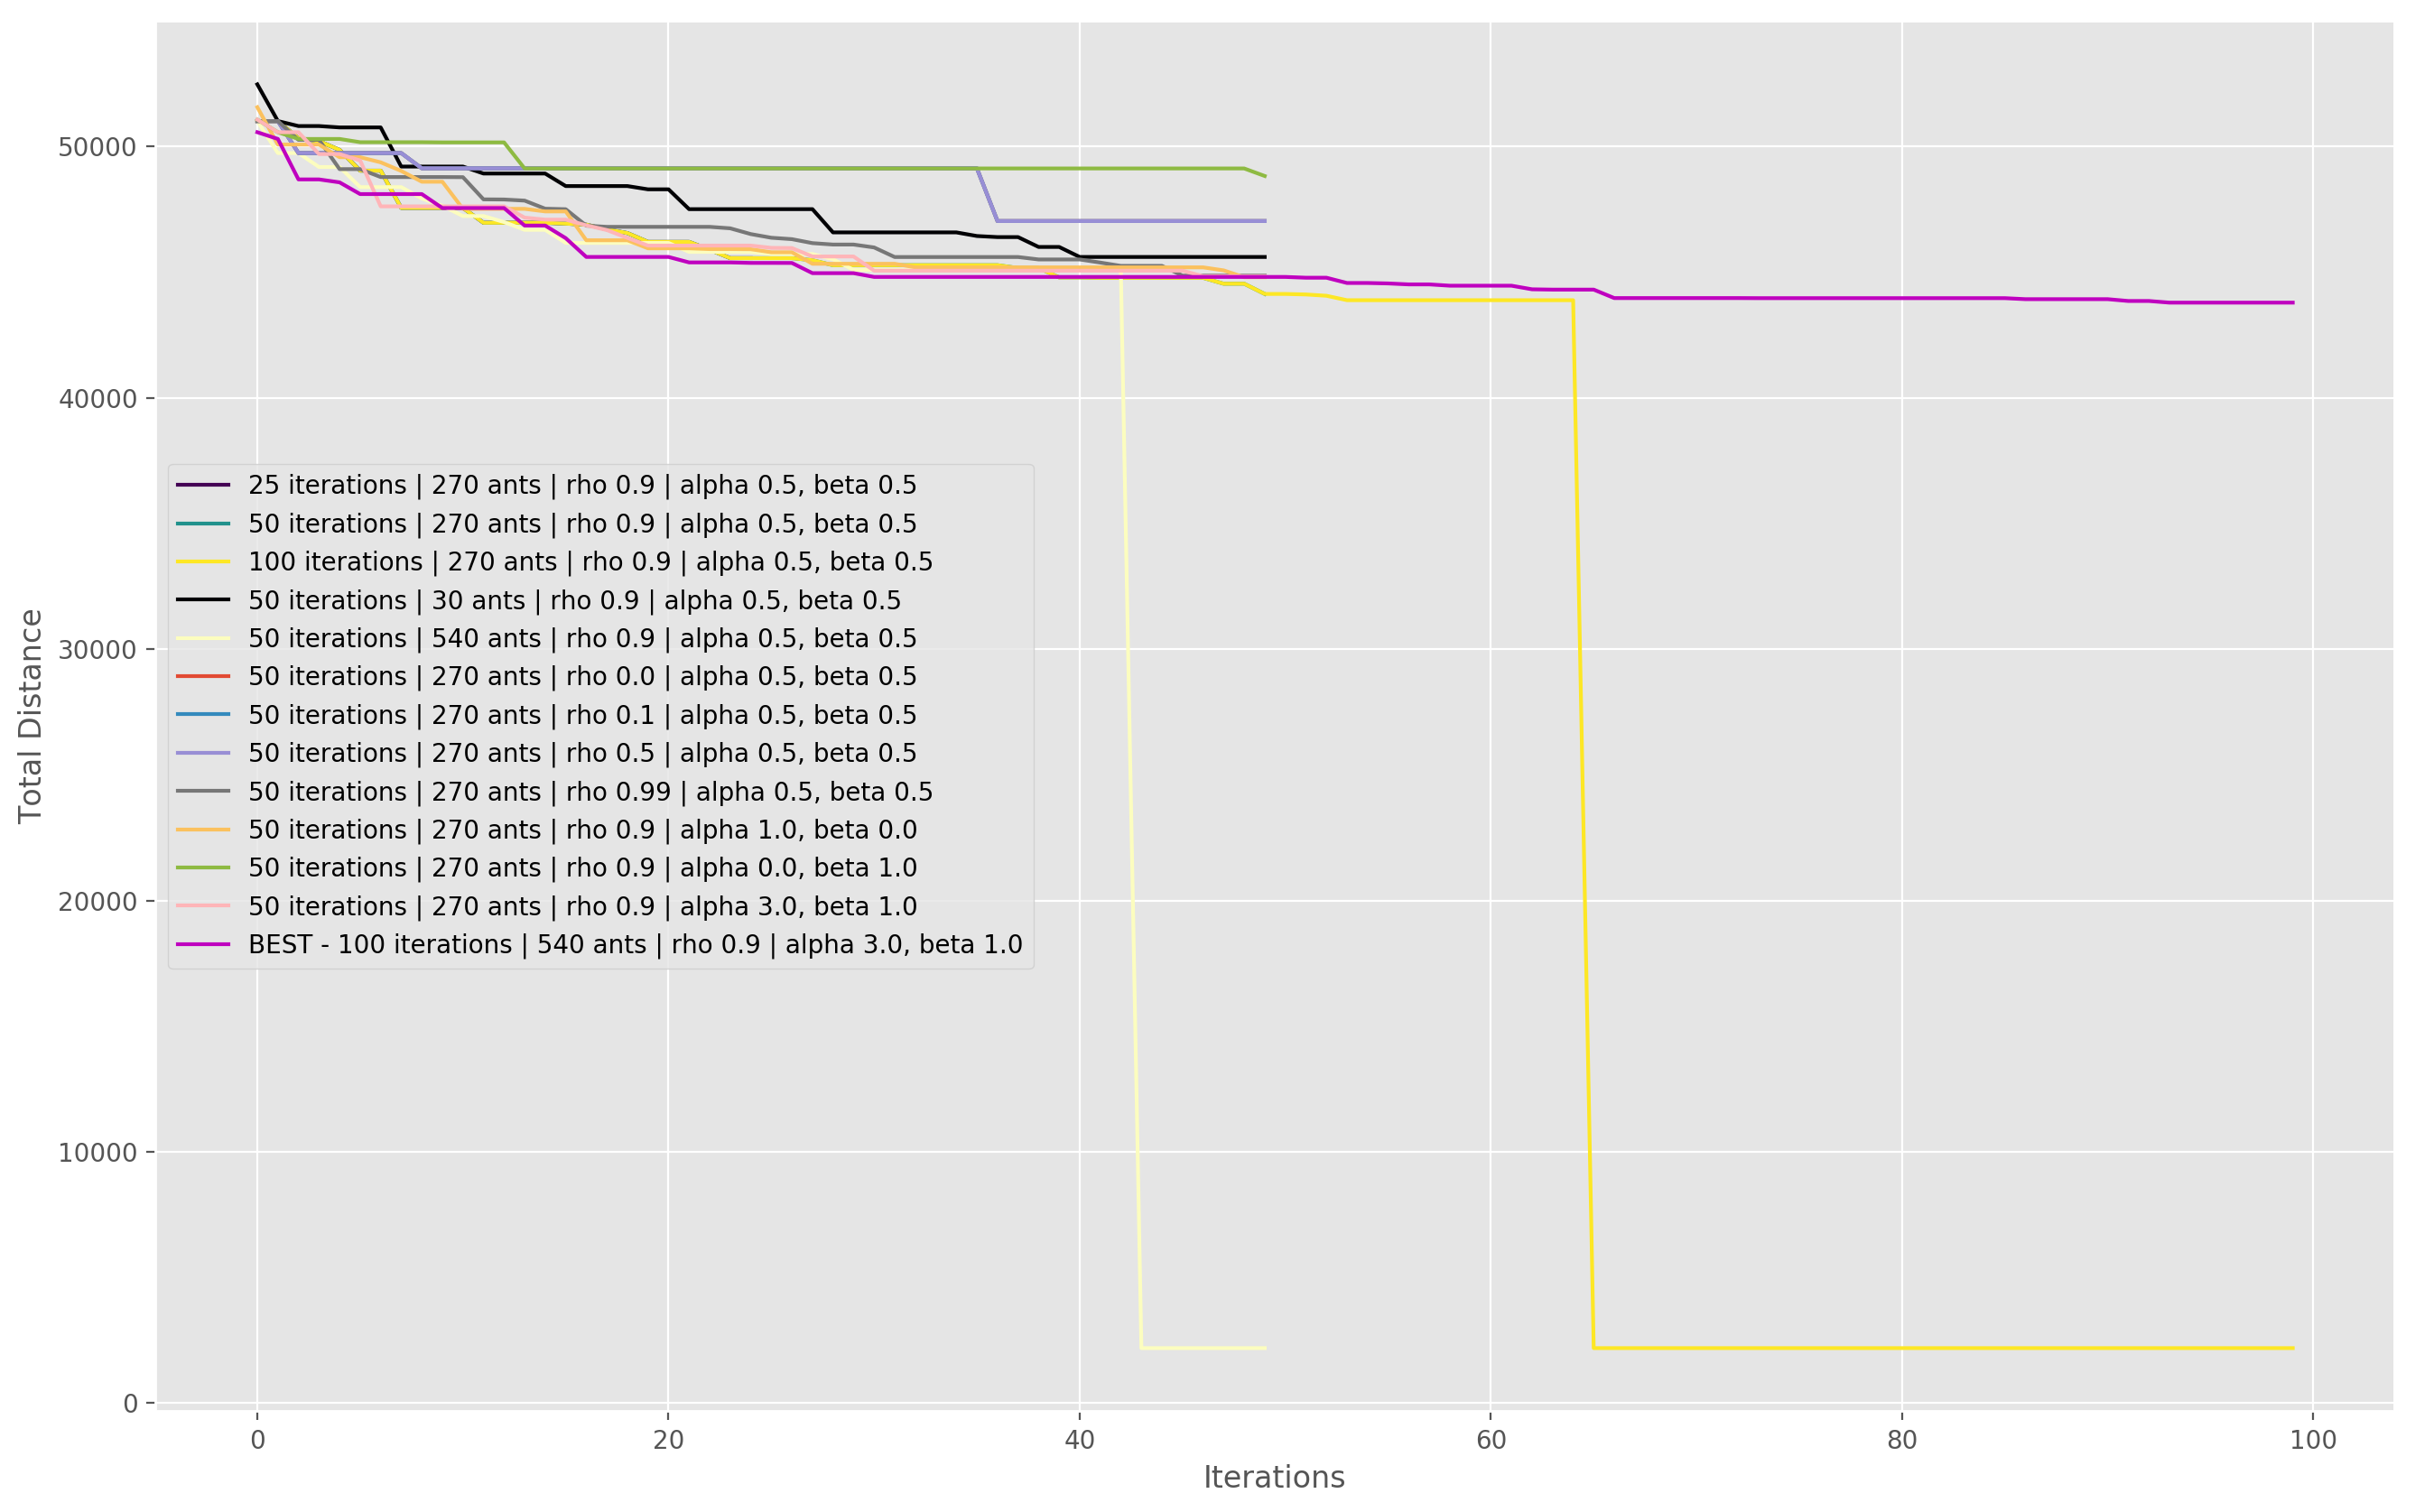
\includegraphics[width=11cm,keepaspectratio]{images/SJC3b_best.png}
  \caption{Melhores soluções encontradas para a base SJC3b ao longo das repetições para todas as variações de parâmetros apresentadas até agora.}
  \label{fig:sjc3b_best}
\end{figure}
\section{Conclusão}

Esse trabalho foi bem interessante por mostrar que da ignorância de um indivíduo sozinho pode surgir a inteligência, quando combinados de maneira a cooperarem. Apesar de ser, em teoria, mais simples do que o algoritmo de programação genética, implementado no último trabalho prático, a implementação deste trabalho foi bem trabalhosa, principalmente devido aos diversos problemas encontrados no artigo que foi usado como base para criação do enunciado.

O principal problema foi o fato de a heurística para solução do \textbf{GAP} proposta no artigo acabar, muitas vezes, gerando soluções inválidas na alocação de nós às medianas, assim gerando resultados melhores do que o possível. Fica a dúvida de se os resultados expostos na seção de avaliação de performance do artigo não são melhores apenas por conta disso, ou se esses problemas não ocorriam nos \textit{datasets} usados pelos autores. De qualquer forma, é triste ver que esse artigo tem 17 citações e o problema nunca foi notado, mesmo 12 anos depois. Por sorte, hoje em dia, principalmente na área de computação evolutiva, muitas vezes a implementação é requerida para dar mais suporte aos artigos à serem publicados.

\bibliographystyle{IEEEannot}
\bibliography{annot}
\end{document}